%Version 3.1 December 2024
% See section 11 of the User Manual for version history
%
%%%%%%%%%%%%%%%%%%%%%%%%%%%%%%%%%%%%%%%%%%%%%%%%%%%%%%%%%%%%%%%%%%%%%%
%%                                                                 %%
%% Please do not use \input{...} to include other tex files.       %%
%% Submit your LaTeX manuscript as one .tex document.              %%
%%                                                                 %%
%% All additional figures and files should be attached             %%
%% separately and not embedded in the \TeX\ document itself.       %%
%%                                                                 %%
%%%%%%%%%%%%%%%%%%%%%%%%%%%%%%%%%%%%%%%%%%%%%%%%%%%%%%%%%%%%%%%%%%%%%

%%\documentclass[referee,sn-basic]{sn-jnl}% referee option is meant for double line spacing

%%=======================================================%%
%% to print line numbers in the margin use lineno option %%
%%=======================================================%%

%%\documentclass[lineno,pdflatex,sn-basic]{sn-jnl}% Basic Springer Nature Reference Style/Chemistry Reference Style

%%=========================================================================================%%
%% the documentclass is set to pdflatex as default. You can delete it if not appropriate.  %%
%%=========================================================================================%%

%%\documentclass[sn-basic]{sn-jnl}% Basic Springer Nature Reference Style/Chemistry Reference Style

%%Note: the following reference styles support Namedate and Numbered referencing. By default the style follows the most common style. To switch between the options you can add or remove “Numbered” in the optional parenthesis. 
%%The option is available for: sn-basic.bst, sn-chicago.bst%  
 
%%\documentclass[pdflatex,sn-nature]{sn-jnl}% Style for submissions to Nature Portfolio journals
%%\documentclass[pdflatex,sn-basic]{sn-jnl}% Basic Springer Nature Reference Style/Chemistry Reference Style
\documentclass[pdflatex,sn-mathphys-num]{sn-jnl}% Math and Physical Sciences Numbered Reference Style
%%\documentclass[pdflatex,sn-mathphys-ay]{sn-jnl}% Math and Physical Sciences Author Year Reference Style
%%\documentclass[pdflatex,sn-aps]{sn-jnl}% American Physical Society (APS) Reference Style
%%\documentclass[pdflatex,sn-vancouver-num]{sn-jnl}% Vancouver Numbered Reference Style
%%\documentclass[pdflatex,sn-vancouver-ay]{sn-jnl}% Vancouver Author Year Reference Style
%%\documentclass[pdflatex,sn-apa]{sn-jnl}% APA Reference Style
%%\documentclass[pdflatex,sn-chicago]{sn-jnl}% Chicago-based Humanities Reference Style

%%%% Standard Packages
%%<additional latex packages if required can be included here>

\usepackage{graphicx}%
\usepackage{multirow}%
\usepackage{amsmath,amssymb,amsfonts}%
\usepackage{amsthm}%
\usepackage{mathrsfs}%
\usepackage[title]{appendix}%
\usepackage{xcolor}%
\usepackage{textcomp}%
\usepackage{manyfoot}%
\usepackage{booktabs}%
\usepackage{algorithm}%
\usepackage{algorithmicx}%
\usepackage{algpseudocode}%
\usepackage{listings}%
\usepackage{placeins}

%%%%

%%%%%=============================================================================%%%%
%%%%  Remarks: This template is provided to aid authors with the preparation
%%%%  of original research articles intended for submission to journals published 
%%%%  by Springer Nature. The guidance has been prepared in partnership with 
%%%%  production teams to conform to Springer Nature technical requirements. 
%%%%  Editorial and presentation requirements differ among journal portfolios and 
%%%%  research disciplines. You may find sections in this template are irrelevant 
%%%%  to your work and are empowered to omit any such section if allowed by the 
%%%%  journal you intend to submit to. The submission guidelines and policies 
%%%%  of the journal take precedence. A detailed User Manual is available in the 
%%%%  template package for technical guidance.
%%%%%=============================================================================%%%%

%% as per the requirement new theorem styles can be included as shown below
\theoremstyle{thmstyleone}%
\newtheorem{theorem}{Theorem}%  meant for continuous numbers
%%\newtheorem{theorem}{Theorem}[section]% meant for sectionwise numbers
%% optional argument [theorem] produces theorem numbering sequence instead of independent numbers for Proposition
\newtheorem{proposition}[theorem]{Proposition}% 
%%\newtheorem{proposition}{Proposition}% to get separate numbers for theorem and proposition etc.

\theoremstyle{thmstyletwo}%
\newtheorem{example}{Example}%
\newtheorem{remark}{Remark}%

\theoremstyle{thmstylethree}%
\newtheorem{definition}{Definition}%

\raggedbottom
%%\unnumbered% uncomment this for unnumbered level heads

\begin{document}

\title[EEG Motor Action and Motor Imagery Classification]{EEG-Based Motor Action and Motor Imagery Classification Using Machine Learning}

\author[1]{\fnm{Harsada} \sur{K}}\email{cb.ai.u4aid24019@cb.students.amrita.edu}
\author[1]{\fnm{V} \sur{Tanay Darshan}}\email{cb.ai.u4aid24059@cb.students.amrita.edu}
\author[1]{\fnm{K} \sur{Nikhitha}}\email{cb.ai.u4aid24042@cb.students.amrita.edu}
\author[1]{\fnm{S Sai} \sur{Tejesh Reddy}}\email{cb.ai.u4aid24057@cb.students.amrita.edu}
\author*[1]{\fnm{Abhishek} \sur{S}}\email{s\_abhishek@cb.amrita.edu}

\affil*[1]{\orgdiv{Amrita School of Artificial Intelligence, Coimbatore}\\ \orgname{Amrita Vishwa Vidyapeetham}, \country{India}}

\abstract{This work presents an EEG-based classification framework for distinguishing motor actions and motor imagery using a consumer-grade Emotiv EPOC X headset. We recorded 14-channel EEG at 128~Hz from 47 participants while they performed, and then imagined, six limb movements (right and left arm, leg and wrist), which gives twelve tasks. Because the task schedule did not start at the same moment in every recording, we located it using the headset's own motion sensor. The signals were band-pass filtered between 4 and 45~Hz, trials with large amplitudes or spikes were removed, and the remaining 476 trials were cut into 8,092 overlapping 2~s windows. Each window was described by 1,771 features covering band power, statistics, fractal measures, wavelets, spectrograms, scalograms, inter-hemispheric connectivity and Riemannian covariance, all standardised within each recording. An ensemble of logistic regression, linear discriminant analysis, extra trees and histogram gradient boosting, trained with left--right mirrored copies of the data, classified the windows, and the windows of a trial were averaged into one decision. Under person-wise GroupKFold validation, the system reached 80.25\% for action versus imagery, 26.68\% for body part (six classes) and 21.43\% for all twelve tasks. Shuffled-label tests fell to chance on every task and repeated runs gave nearly identical results. Left versus right imagery reached 58.09\% in standard cross-validation but only 52.28\% under nested cross-validation, so it could not be decoded reliably. Adding common spatial pattern features changed the ensemble's accuracy by less than two points in either direction.}

\keywords{Electroencephalography (EEG), Brain--Computer Interface, Motor Imagery, Motor Action, Spectrogram, Scalogram, Riemannian Geometry, Machine Learning, Emotiv EPOC X}

\maketitle

%% ===================================================================
\section{Introduction}\label{sec1}

A brain--computer interface (BCI) reads patterns of brain activity and turns them into commands for a computer or a device. Motor applications are where this matters most. A person who cannot move a limb may still produce the cortical activity that normally comes before a movement, and a BCI that picks up this activity could drive a prosthesis, a wheelchair or a rehabilitation robot. Electroencephalography (EEG) is the usual signal for such systems because it is non-invasive, follows brain activity at the millisecond scale and can be recorded with portable equipment \citep{Wolpaw2002,NicolasAlonso2012}.

Two related conditions are of interest here. In motor execution, or \emph{action}, the person really moves. In motor imagery the person rehearses the same movement in their head and stays still. Both conditions change the sensorimotor rhythms, mostly in the mu (8--12~Hz) and beta (13--30~Hz) bands, and these changes are what most motor-imagery BCIs rely on \citep{Pfurtscheller2001,PfurtschellerAranibar1977}.

Early systems kept the problem small, typically left- versus right-hand imagery, and solved it with Common Spatial Pattern (CSP) filters followed by an LDA or SVM classifier \citep{Ramoser2000,Blankertz2008}. Things get much harder once more body parts or conditions are added. The cortical areas for different limbs sit close together, the skull smears their activity across the scalp, and the EEG of one person can look quite different from that of the next \citep{Naeem2006,Lotte2018}.

Hardware adds its own limits. Clinical amplifiers give clean signals but are costly and slow to set up. Consumer headsets such as the Emotiv EPOC are cheap and quick to wear, and they do capture real neural activity, but they are noisier, more sensitive to movement and have fewer electrodes \citep{Badcock2013,Duvinage2013,Maskeliunas2016}.

Researchers have tried several ways of describing EEG to get around these problems. Spectral and time--frequency features capture how rhythms change during a task. Riemannian methods describe each trial by the covariance between its channels and work with the geometry of these matrices \citep{Barachant2012,Congedo2017}. Deep networks such as EEGNet learn their own features from the raw signal \citep{Schirrmeister2017,Lawhern2018}. None of these views is likely to capture everything in a few seconds of EEG, so combining them seems sensible.

In this study we built a complete pipeline around the 14-channel Emotiv EPOC X and a twelve-task protocol: six movements (right and left arm, leg and wrist), each performed once as an action and once as imagery. We analysed the same recordings at three levels of detail: action versus imagery (two classes), body part (six classes) and the exact task (twelve classes). At our guide's suggestion we also tried to decode the side of an imagined movement. Every result is subject-independent, meaning the model is always tested on people it has never seen.

The main contributions of this work are:

\begin{enumerate}
\item \textbf{A twelve-task motor dataset recorded with consumer-grade EEG.} We recorded 47 participants with a 14-channel Emotiv EPOC X while they performed and imagined six limb movements, which gives twelve task conditions per session.

\item \textbf{Multi-level motor classification.} The same trials are classified as action or imagery, by body part and by exact task, so the drop in accuracy can be followed as the target becomes more specific.

\item \textbf{Time--frequency and multi-domain feature fusion.} Handcrafted spectral, statistical, fractal and wavelet features are combined with spectrogram (STFT), scalogram (CWT), connectivity and Riemannian tangent-space features, and the value of each family is measured on its own.

\item \textbf{Cross-subject adaptation and trial-level decisions.} Features are standardised within each recording without using labels, the training data are doubled by hemispheric mirroring, and a four-model ensemble makes one decision per trial by averaging its windows.

\item \textbf{A careful check of the results.} Besides person-wise validation, we report shuffled-label tests on all tasks, repeated runs with different random seeds, nested cross-validation, sensitivity to the trial timing and a model-by-model test of whether CSP features help.
\end{enumerate}

Section~\ref{sec:related} reviews related work. Section~\ref{sec:methods} describes the protocol, preprocessing, features, classifiers and evaluation. Section~\ref{sec:results} presents and discusses the results, and Section~\ref{sec:conclusion} concludes.

\FloatBarrier
%% ===================================================================
\section{Literature Review}\label{sec:related}

Decoding movement from EEG has been studied for decades, and the main obstacle has always been the same: scalp EEG has a low signal-to-noise ratio and varies a great deal between trials and between people. The rhythms most closely tied to movement are the mu rhythm (8--12~Hz) and the beta rhythm (13--30~Hz). Their power falls when a movement is made or imagined and comes back afterwards, a pattern called event-related desynchronisation and synchronisation (ERD/ERS). Nearly all motor decoding builds on it \citep{PfurtschellerAranibar1977,PfurtschellerLopes1999}.

CSP has probably been the most influential single method. Ramoser et al.\ showed that spatial filters which maximise the difference in variance between two classes work well for two-class motor imagery \citep{Ramoser2000}. Blankertz et al.\ later explained how to make such filters hold up against noise and small training sets \citep{Blankertz2008}. Filter-bank CSP (FBCSP) added the observation that the most useful frequencies differ from person to person, so it runs CSP in several sub-bands and selects the best features \citep{Ang2012}. FBCSP won the BCI Competition IV and is still a standard baseline.

Covariance-based methods grew out of the limits of spatial filtering. Barachant et al.\ treated the covariance matrix of each trial as a point on the manifold of symmetric positive-definite matrices and classified trials by their Riemannian distance to class means \citep{Barachant2012}. Projecting these matrices onto a tangent space lets ordinary classifiers use them while keeping their structure. Riemannian methods have since become a strong choice for multi-class EEG, especially when people differ a lot \citep{Congedo2017}.

Time--frequency analysis looks at the same signals from another angle. ERD/ERS unfolds over time, so averaging power over a whole window can hide it. The short-time Fourier transform (STFT) gives a spectrogram that shows how band power changes, and Tabar and Halici fed STFT images to a convolutional network for motor imagery \citep{Tabar2017}. The continuous wavelet transform (CWT) gives a scalogram instead. It analyses high frequencies with short windows and low frequencies with long ones, a better trade-off for signals whose rhythms come and go \citep{Torrence1998}.

Deep learning is another major line of work. Convolutional networks learn spatial and temporal filters straight from raw EEG \citep{Schirrmeister2017}, and Sakhavi et al.\ added a temporal filter-bank representation to capture how the signal evolves \citep{Sakhavi2018}. EEGNet showed that a compact network built from depthwise and separable convolutions can compete with much larger models while using far fewer parameters \citep{Lawhern2018}.

Generalising to new people remains hard. EEG distributions shift between people because of anatomy, electrode position, amplitude and the way each person does the imagery. Alignment methods reduce this shift by re-centring each person's data before classification, either in Euclidean space \citep{He2020} or on the Riemannian manifold \citep{Zanini2018,Zhang2020}. Reviews of deep learning for EEG also point out that its gains are uneven when training data are scarce or recordings differ from benchmark datasets \citep{Roy2019,Altaheri2023}.

Consumer-grade EEG lowers the cost barrier but brings signal-quality problems of its own. Studies with Emotiv devices show that task-related activity can be recovered, though with more variability and lower spatial resolution than research systems \citep{Badcock2013,Duvinage2013,Maskeliunas2016}. Motor-imagery BCIs have nonetheless reached clinical use, for example in robot-assisted stroke rehabilitation \citep{Ang2015}.

Most motor-imagery studies deal with two or four classes recorded with research-grade equipment on benchmark datasets. Separating several body parts, and real from imagined movement, is much less explored, particularly with a low-cost headset. This gap motivated our study: we ask several related questions of the same recordings and combine time--frequency, handcrafted and covariance features under subject-independent validation. Table~\ref{tab:litreview} summarises representative studies.

\begin{table*}[t]
\centering
\caption{Representative studies on EEG-based motor imagery and related classification. N/R: not reported in a directly comparable form.}
\label{tab:litreview}
\footnotesize
\setlength{\tabcolsep}{2.5pt}
\begin{tabular}{@{}p{0.06\linewidth}p{0.15\linewidth}p{0.13\linewidth}p{0.17\linewidth}p{0.12\linewidth}p{0.12\linewidth}p{0.16\linewidth}@{}}
\toprule
Ref. & Task / Classes & Dataset / Hardware & Features / Representation & Model & Accuracy & Main Limitation \\
\midrule
\cite{Ramoser2000} & Left vs.\ right hand MI (2-class) & Research EEG, 3 subjects & CSP + log-variance & LDA & $\approx$80--90\% & Restricted to binary MI \\ \addlinespace
\cite{Blankertz2008} & Binary motor imagery & Research EEG & CSP and regularised variants & LDA & N/R & Mainly binary; needs parameter tuning \\ \addlinespace
\cite{Naeem2006} & Hand, foot, tongue (4-class) & Research EEG & ICA-based representation & LDA & N/R & Limited spatial separability \\ \addlinespace
\cite{Ang2012} & Motor imagery (4-class) & BCI Competition IV-2a & Filter-bank CSP + feature selection & Naive Bayes & $\approx$68\% & Many frequency/filter parameters \\ \addlinespace
\cite{Barachant2012} & Multi-class MI & Research EEG & Covariance matrices + Riemannian geometry & MDM / tangent-space classifier & N/R & Costly covariance operations \\ \addlinespace
\cite{Schirrmeister2017} & Motor imagery (4-class) & BCI Competition IV-2a & Learned spatio-temporal features & Deep / Shallow ConvNet & $\approx$71--74\% & Data-hungry, less interpretable \\ \addlinespace
\cite{Lawhern2018} & Several BCI paradigms & Public EEG datasets & Depthwise and separable convolutions & EEGNet & N/R & Needs enough training data \\ \addlinespace
\cite{Tabar2017} & Motor imagery (2-class) & BCI Competition IV-2b & STFT images & CNN + stacked autoencoder & $\approx$77\% & Complex, data-sensitive training \\ \addlinespace
\cite{Sakhavi2018} & Motor imagery (4-class) & BCI Competition IV-2a & Temporal filter-bank representation & CNN & $\approx$74.5\% & More complex architecture \\ \addlinespace
\cite{He2020} & Cross-subject MI/ERP & Public EEG datasets & Euclidean alignment of covariance & Various classifiers & N/R & Assumes a moderate covariance shift \\ \addlinespace
\cite{Zanini2018} & Cross-subject MI & Public EEG datasets & Riemannian re-centring of covariances & MDM & N/R & Needs unlabelled data of the new subject \\ \addlinespace
\cite{Zhang2020} & Cross-subject EEG & Four EEG datasets & Riemannian alignment + tangent space & MEKT & N/R & Needs source/target adaptation \\ \addlinespace
\cite{Badcock2013} & EEG signal validation & Emotiv EPOC (14-ch) & Auditory event-related potentials & ERP analysis & N/R & Lower spatial resolution than clinical EEG \\ \addlinespace
\cite{Maskeliunas2016} & Concentration / blink control & Emotiv EPOC, NeuroSky & EEG control features & Conventional classifiers & N/R & High inter-trial variability \\ \addlinespace
\cite{Ang2015} & MI-based stroke rehabilitation & Stroke patients & CSP-based MI features & BCI + robotic feedback & N/R & Small clinical cohort \\ \addlinespace
\textbf{Our work} & Action vs.\ imagery (2), body part (6), full task (12), left vs.\ right imagery (2) & Emotiv EPOC X (14-ch, 128 Hz), 47 participants & 1,771 features: handcrafted + STFT + CWT + connectivity + Riemannian & Ensemble (LR + LDA + Extra Trees + HistGB), mirror augmentation, trial-level voting & 80.25\% (2-class); 26.68\% (6-class); 21.43\% (12-class); L/R not above chance in nested CV & Consumer EEG; limb and side remain hard to decode across people \\
\botrule
\end{tabular}
\end{table*}
\FloatBarrier

%% ===================================================================
\section{Proposed Methodology}\label{sec:methods}

\subsection{System Overview}\label{subsec:overview}

The system takes the raw recordings from the headset and returns one label for every 10~s task. Fig.~\ref{fig:pipeline} shows the two stages of the processing chain.

The first stage, \emph{signal preparation}, turns a continuous recording into clean, labelled trials. It finds where the task schedule starts using the headset's motion sensor, band-pass filters the EEG, cuts out the twelve trials, discards trials with artefacts and normalises each recording. Each trial is then split into short overlapping windows.

The second stage, \emph{representation and classification}, describes every window with spectral, time--frequency, statistical, connectivity and covariance features, standardises them within each recording and classifies each window with an ensemble of four models. The predictions for the windows of one trial are averaged into a single decision. Throughout, no person's data are ever used for training and testing in the same fold.

\begin{figure}[htbp]
\centering
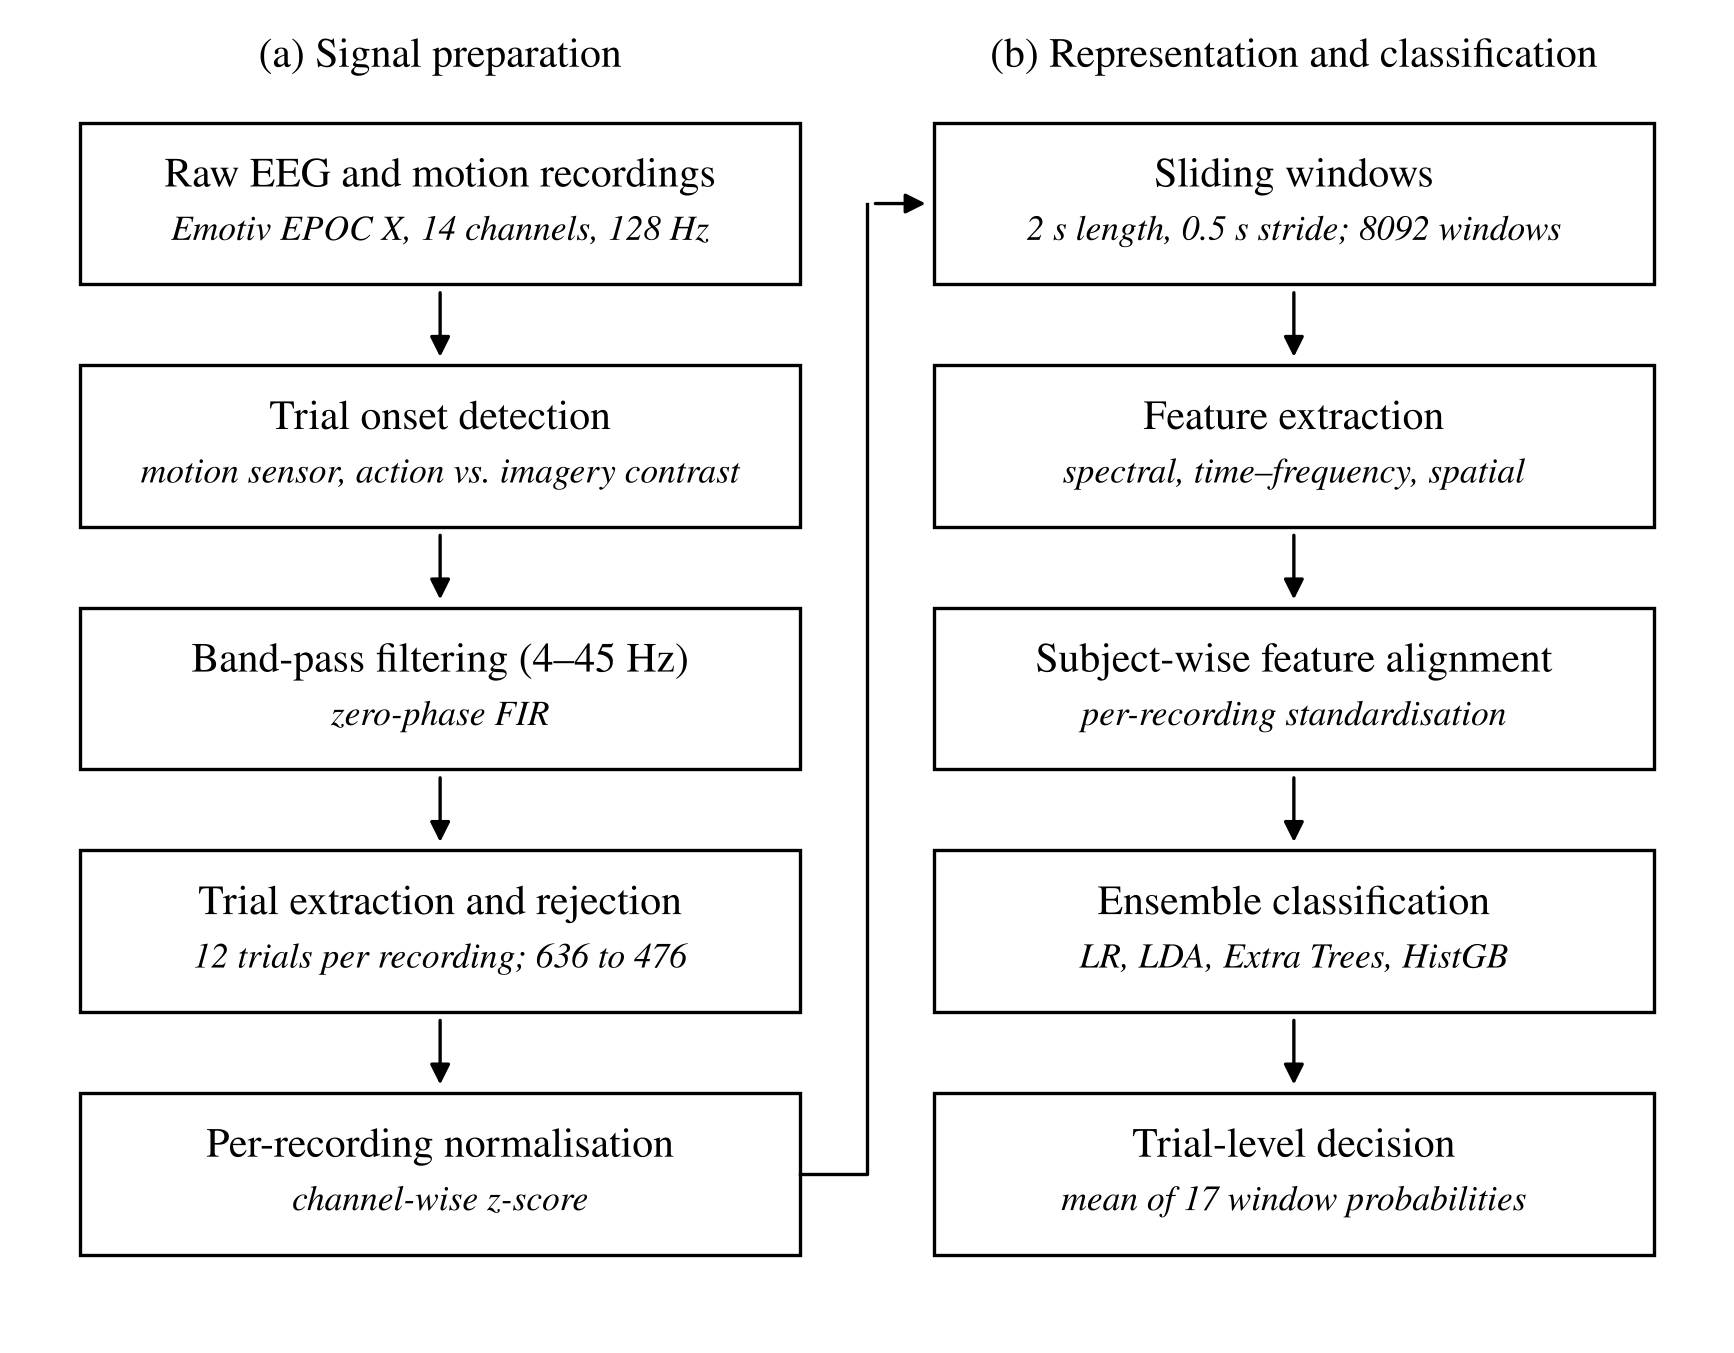
\includegraphics[width=0.85\textwidth]{figures/fig1_pipeline.png}
\caption{Overview of the proposed pipeline. (a) Signal preparation; (b) representation and classification.}
\label{fig:pipeline}
\end{figure}

\subsection{Experimental Protocol}\label{subsec:protocol}

Participants sat in front of a screen in a quiet room. They kept their eyes open, followed the instruction on the screen, avoided needless movement and speech, and relaxed whenever a fixation cross appeared. The protocol covers six movements: right-arm flexion, left-arm flexion, right-leg lift, left-leg lift, right-wrist rotation and left-wrist rotation. Each movement is first made for real (\emph{action}) and then rehearsed mentally without moving (\emph{imagery}), giving twelve tasks in a fixed order:
\begin{verbatim}
RightArm_Action    RightArm_Imagine
LeftArm_Action     LeftArm_Imagine
RightLeg_Action    RightLeg_Imagine
LeftLeg_Action     LeftLeg_Imagine
RightWrist_Action  RightWrist_Imagine
LeftWrist_Action   LeftWrist_Imagine
\end{verbatim}
Each task lasts 10~s and is followed by 5~s of rest, so the whole schedule takes 175~s from the start of the first task to the end of the last. The dataset contains two session layouts (Fig.~\ref{fig:protocol}). In most sessions the schedule began a few seconds after the recording started. In several later sessions the recording opened with a resting baseline, about 50~s with eyes open and 50~s with eyes closed, so the tasks started roughly two minutes in. Every trial carries three labels: the task (12 classes), the condition, action or imagery (2 classes), and the body part (6 classes).

\begin{figure}[htbp]
\centering
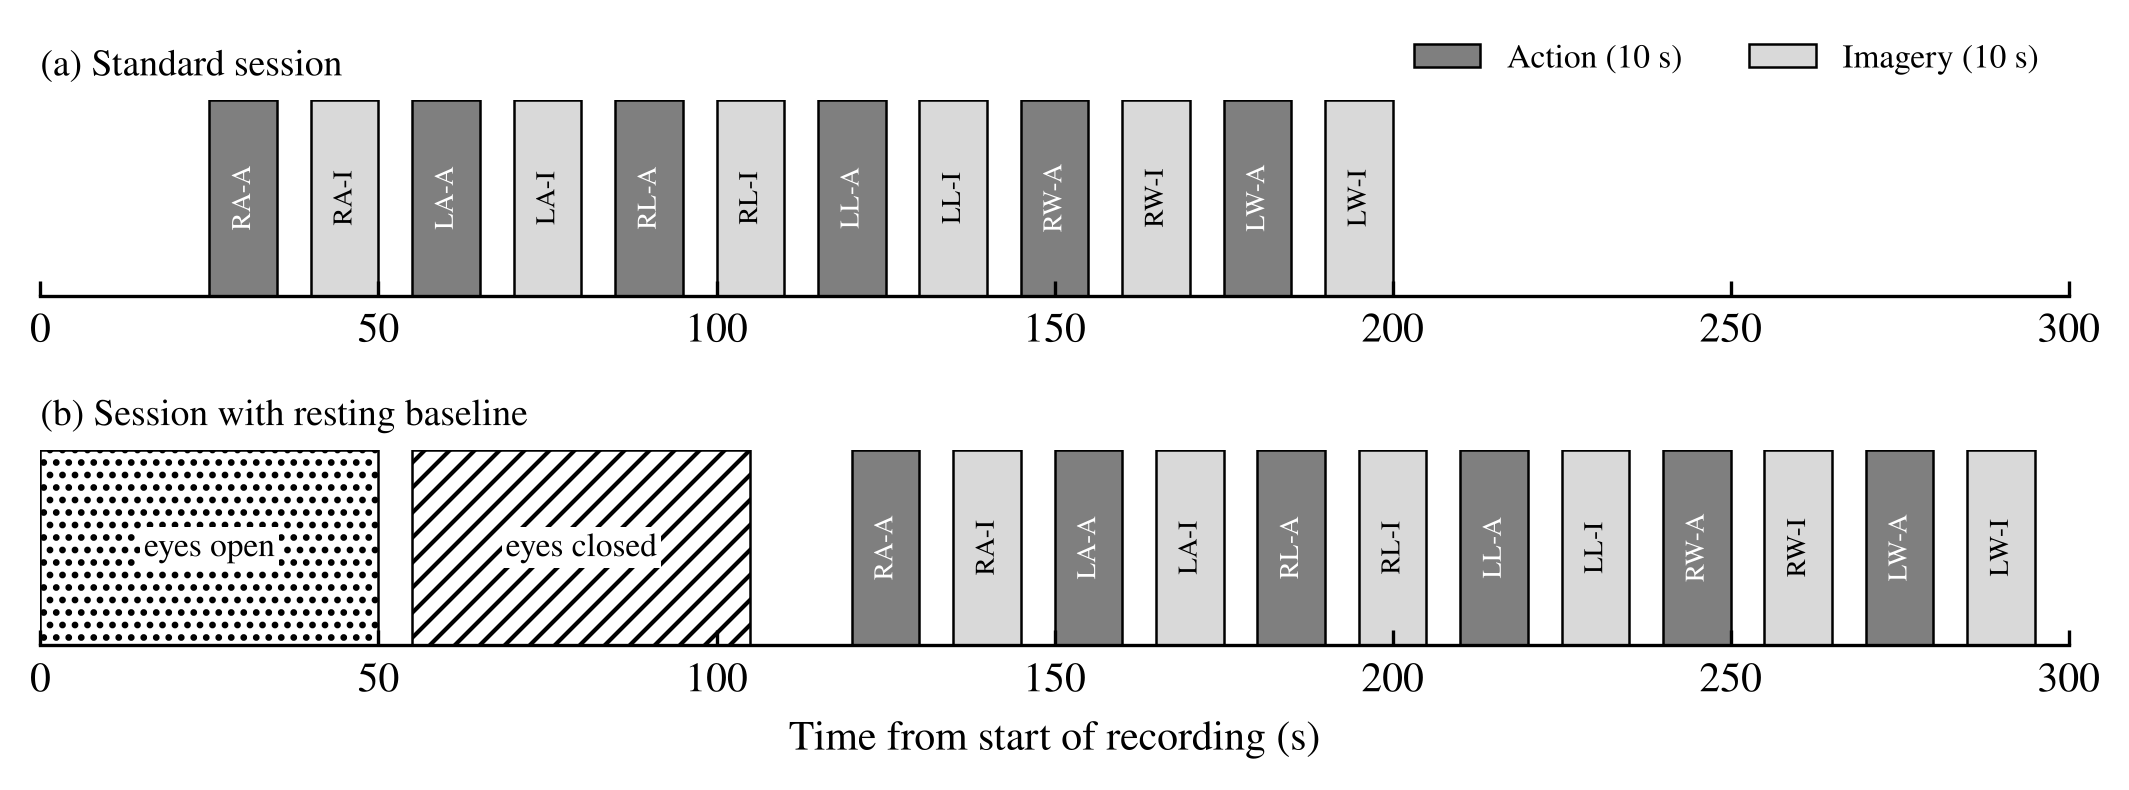
\includegraphics[width=\textwidth]{figures/fig2_protocol.png}
\caption{Timeline of a recording session. (a) Standard session; (b) session with an eyes-open/eyes-closed baseline. RA/LA, RL/LL and RW/LW denote right/left arm, leg and wrist; A = action, I = imagery.}
\label{fig:protocol}
\end{figure}

\subsection{Data Acquisition}\label{subsec:acquisition}

EEG was recorded with a 14-channel Emotiv EPOC X fitted with saline-soaked felt electrodes at AF3, AF4, F3, F4, F7, F8, FC5, FC6, T7, T8, P7, P8, O1 and O2, following the international 10--20 system and using the headset's CMS/DRL reference. The signals were sampled at 128~Hz and saved in EDF format by the EmotivPRO software. For every session, EmotivPRO also stores a second file from the headset's inertial sensor, with three accelerometer axes and four quaternion (orientation) components sampled at 32~Hz. We never used this motion file for classification, only to locate the task schedule (Section~\ref{subsec:onset}). In total we collected 59 EEG recordings with all fourteen channels from 47 participants; a few people were recorded in more than one session.

\subsection{Motion-Guided Trial Onset Detection}\label{subsec:onset}

To cut the trials correctly we need to know when the first task begins in each recording. Our first pipeline simply assumed a 15~s delay for every recording. When we checked this against the data it turned out to be wrong. The delay between starting the recording and starting the tasks varied from session to session and was over two minutes in sessions with a baseline. With a fixed offset, most trials were cut several seconds too early, so a window labelled with one task often contained the end of the previous one.

To recover the real onset we used a simple observation: moving an arm, a leg or a wrist shakes the head slightly, and the headset's motion sensor picks this up, while imagining the movement does not. The procedure has four steps.

\emph{Step 1: motion energy.} The motion signal is split into 0.5~s bins. For each bin $b$, motion energy is the log of the total absolute change across the seven inertial channels,
\begin{equation}
m_b = \log \sum_{c=1}^{7} \sum_{n \in b} \left| s_c[n] - s_c[n-1] \right|,
\end{equation}
and the sequence $m_b$ is centred on its median and divided by its standard deviation.

\emph{Step 2: scoring each candidate onset.} For every candidate onset $t_0$, in 0.5~s steps, the twelve-task schedule is laid over the motion signal. We take the mean motion energy over seconds 1--10 of each task, skipping the first second while the participant reacts to the cue. For each of the six action--imagery pairs we compute the difference $d_k$, and from these a paired $t$-statistic:
\begin{equation}
d_k = \bar{m}_{\mathrm{action},k} - \bar{m}_{\mathrm{imagery},k}, \qquad
t(t_0) = \frac{\bar{d}}{s_d/\sqrt{6}}, \qquad k = 1,\dots,6.
\end{equation}

\emph{Step 3: choosing the onset.} The candidate with the largest $t$ wins. We call it \emph{confident} if $t \ge 4$ and all six pairs show more motion during action than during imagery.

\emph{Step 4: an independent check.} Recordings were normally stopped soon after the last task, and in the confident recordings the recording ended a median of 181~s after the first task began. This gives a second estimate of the onset, $\hat{t}_0 = T_{\mathrm{rec}} - 181$, which uses neither motion nor labels. An onset that fails Step~3 is still accepted if it lies within 5~s of this estimate. Otherwise the recording is dropped, since mislabelled trials would do more harm than a smaller dataset.

Fig.~\ref{fig:onset} shows the procedure for one recording. Motion energy rises clearly in every action block and stays low during imagery. The $t$-statistic peaks sharply at the detected onset of 26.0~s, while at the old fixed onset of 15~s it is slightly negative. Under the old timing, the ``action'' windows of this recording actually contained \emph{less} movement than the ``imagery'' windows.

\begin{figure}[htbp]
\centering
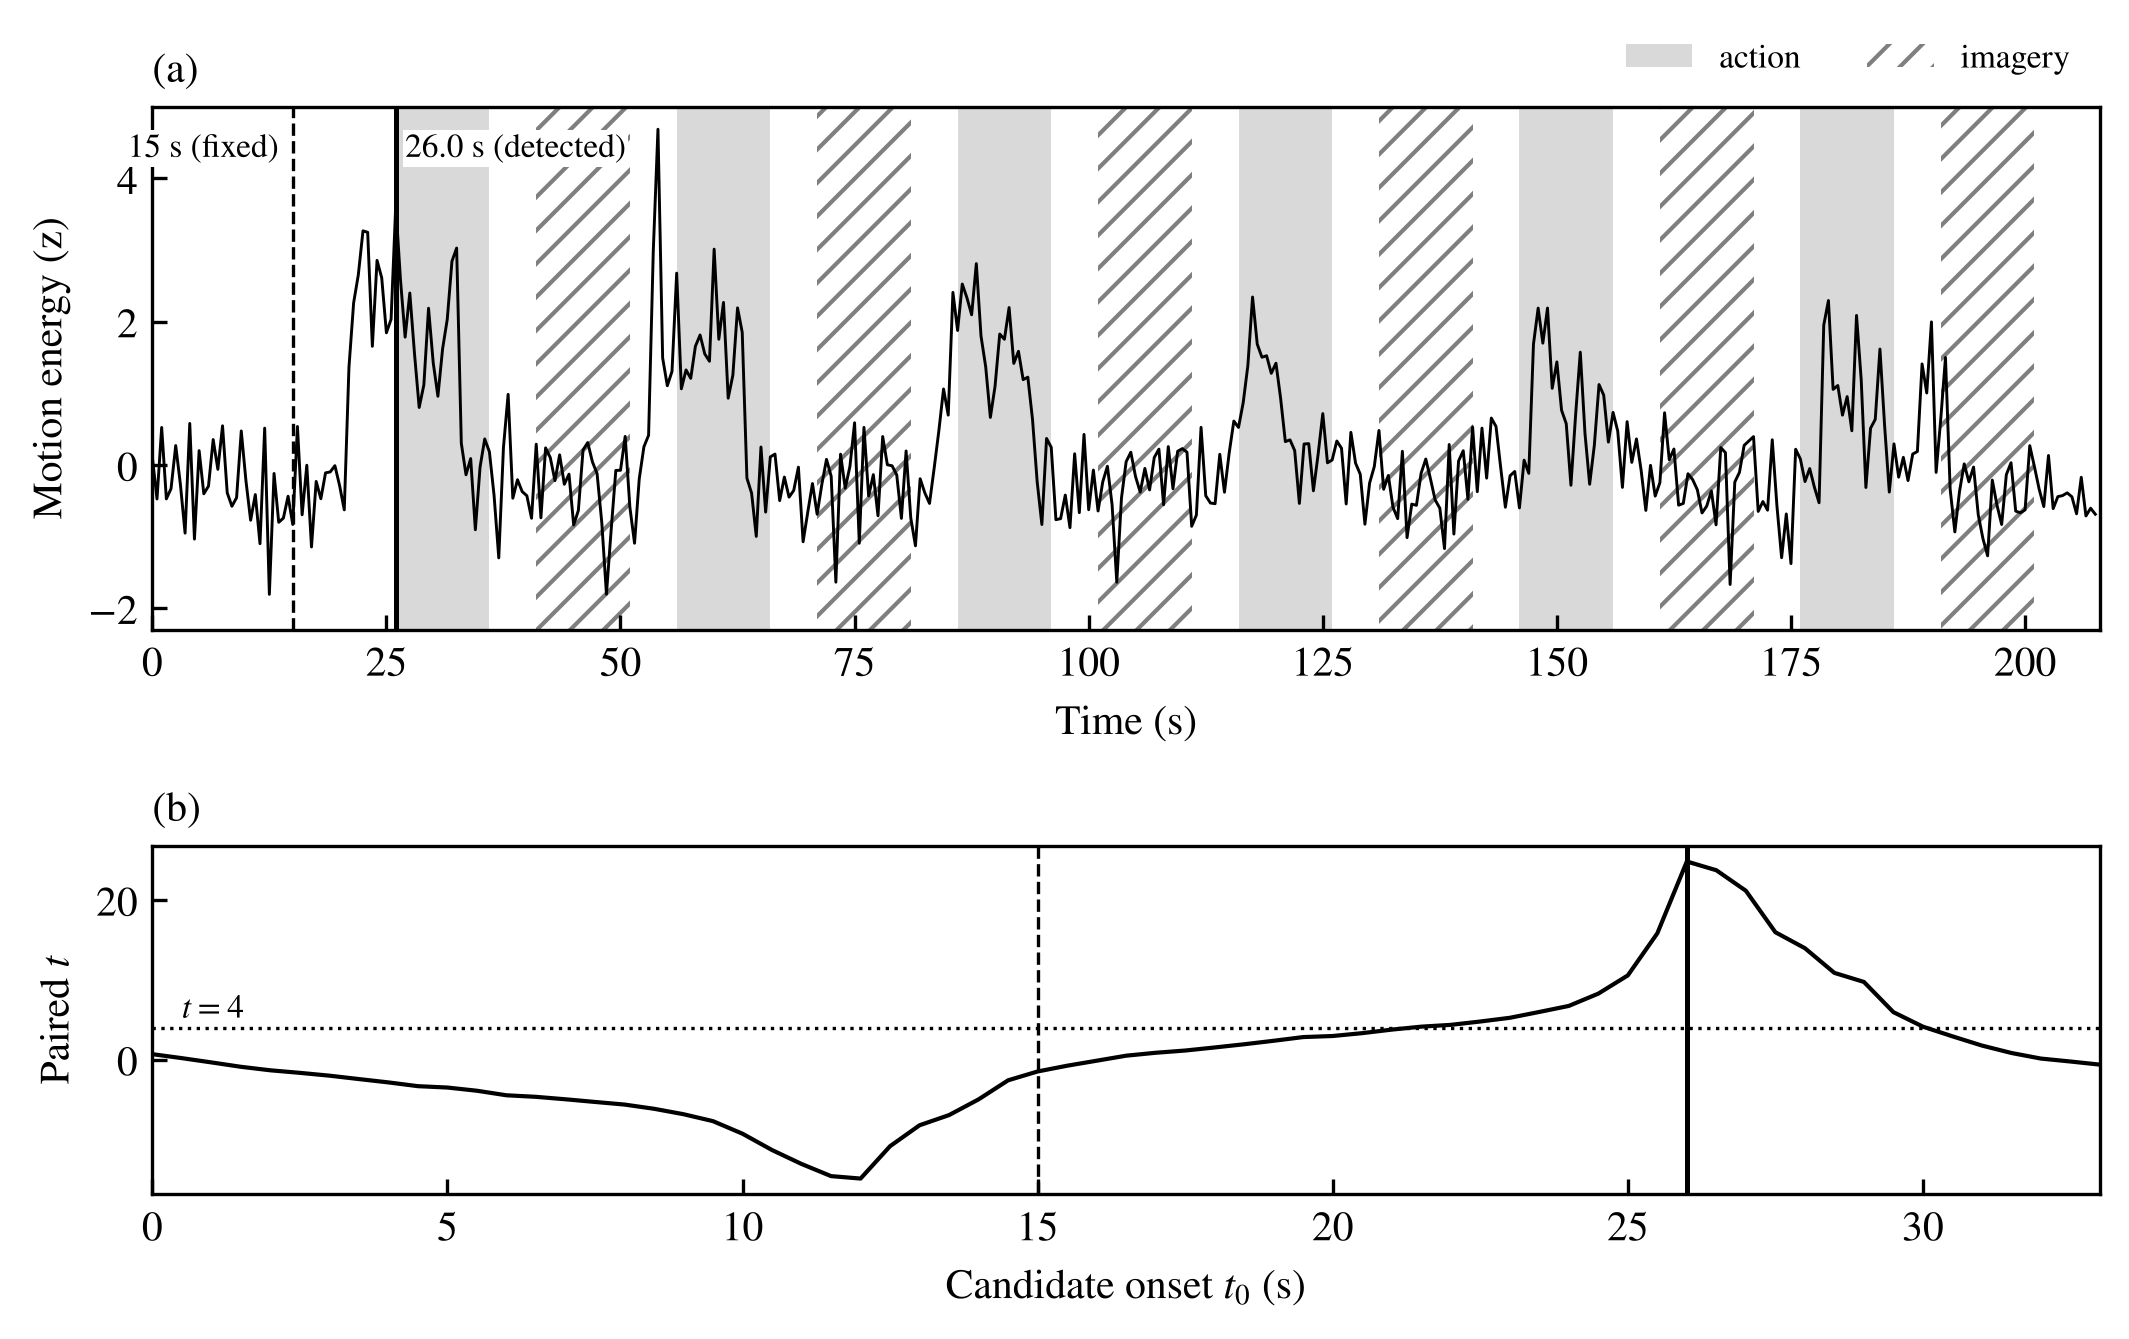
\includegraphics[width=\textwidth]{figures/fig3_onset_detection.png}
\caption{Motion-guided onset detection for one recording. (a) Head-motion energy with the detected schedule; (b) paired $t$-statistic for each candidate onset.}
\label{fig:onset}
\end{figure}

Over the whole dataset, 48 of the 59 recordings gave a confident onset and 5 more passed the duration check. Two were excluded because the two estimates disagreed, and four were too short to hold a complete schedule (sessions that had been stopped and restarted). The detected onsets ranged from 7.5~s to 136.5~s, and the median gap between the motion-based and duration-based estimates was 2.5~s. In the seven sessions where the eyes-closed baseline could be confirmed by a clear rise in occipital alpha power, the detected onset fell 7.3--15.5~s after the end of the eyes-closed period, which is where the schedule should start. The remaining \textbf{53 recordings} were used from here on.

\subsection{Signal Cleaning and Normalisation}\label{subsec:cleaning}

Cleaning has three parts: filtering, trial rejection and normalisation (Fig.~\ref{fig:cleaning}).

\begin{figure}[htbp]
\centering
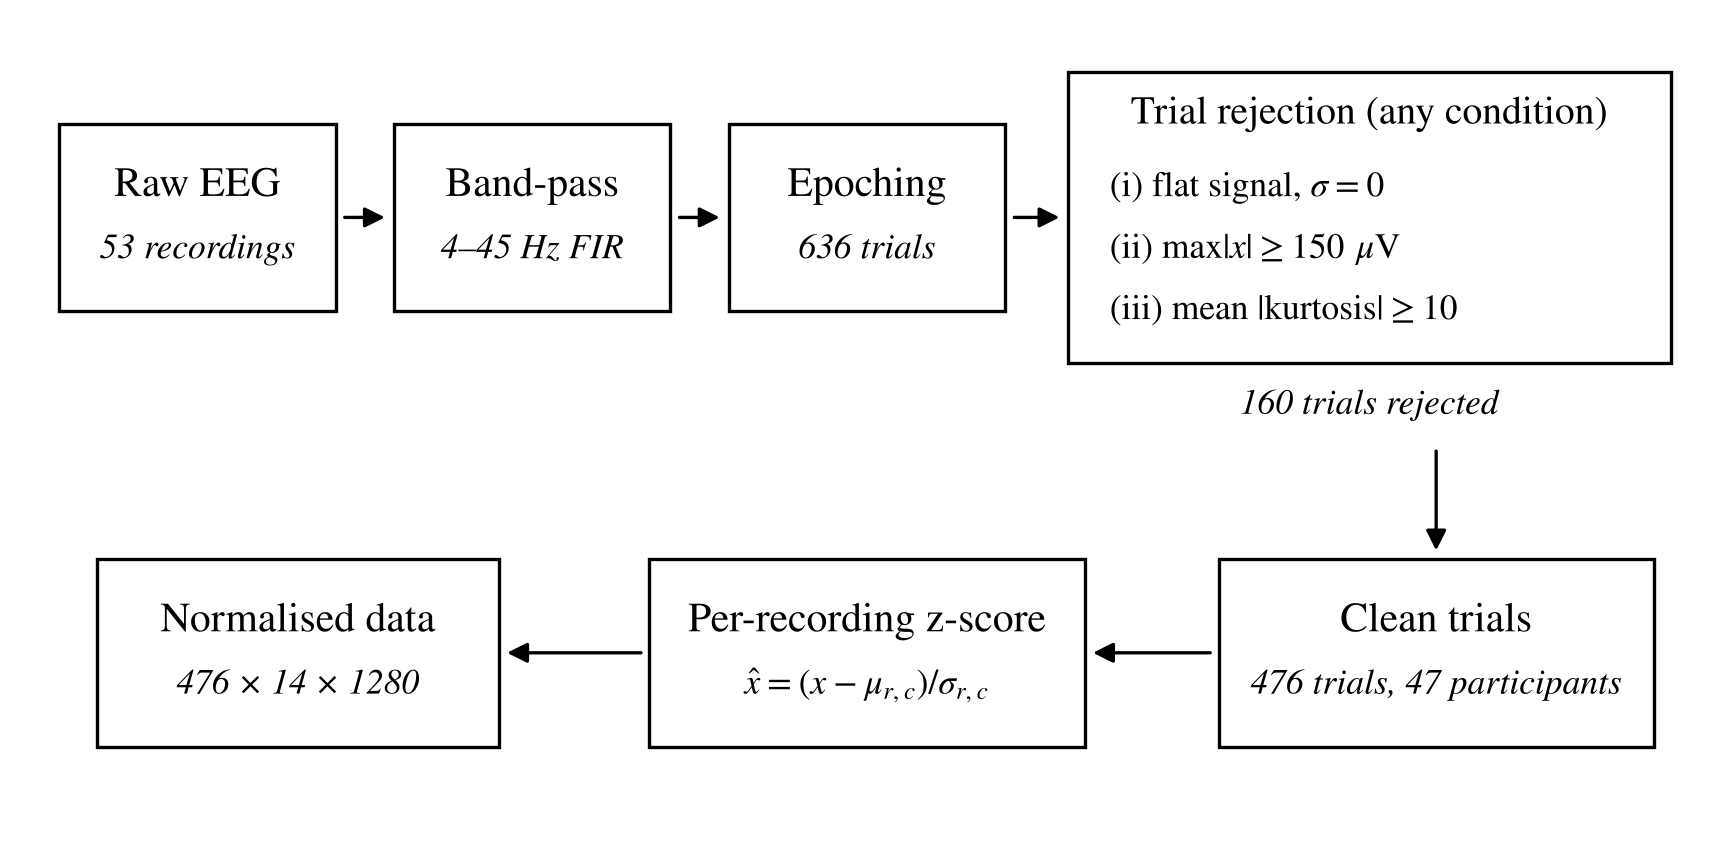
\includegraphics[width=0.9\textwidth]{figures/fig4_cleaning.png}
\caption{Signal cleaning and normalisation.}
\label{fig:cleaning}
\end{figure}

\emph{Band-pass filtering.} The recordings were loaded with MNE-Python \citep{Gramfort2013} and reduced to the fourteen EEG channels; quality, battery and marker channels were dropped and missing samples set to zero. Each continuous recording was filtered between 4 and 45~Hz with a zero-phase FIR filter (Hamming-window design, MNE defaults). The 4~Hz edge removes slow electrode drift and most of the energy of blinks and eye movements. The 45~Hz edge removes high-frequency muscle activity and the 50~Hz mains interference. What remains covers the theta, mu, beta and low-gamma rhythms. A zero-phase filter does not shift the signal in time, and filtering the whole recording before cutting trials avoids edge effects.

\emph{Trial extraction.} Starting from the detected onset $t_0$, trial $k$ ($k = 0,\dots,11$) runs from $t_0 + 15k$ to $t_0 + 15k + 10$~s. Each trial is a $14 \times 1280$ matrix, and the 53 recordings give 636 trials.

\emph{Trial rejection.} A trial was removed if it failed any of three checks: (i) it was flat, with zero variance over the whole trial; (ii) any sample reached 150~$\mu$V, a level genuine EEG on this device stays well below (the median peak of a trial was 92~$\mu$V) and which nearly always means a blink, a jaw clench or a moving cable; or (iii) the mean absolute excess kurtosis across channels was 10 or more, which catches sudden spikes and electrode pops that stay under the amplitude limit. No trial was flat. The amplitude rule caught 158 trials and the kurtosis rule 29, with 27 caught by both, so 160 trials (25.2\%) were removed. That left \textbf{476 clean trials} from 51 recordings and 47 participants. We rejected trials before windowing so that a noisy trial could not slip into training as many overlapping windows. The classes stayed balanced, with 235 action and 241 imagery trials and between 36 and 44 trials for each of the twelve tasks.

\emph{Per-recording normalisation.} Signal amplitude changes between sessions with electrode impedance, the amount of saline and head shape. We therefore z-scored every channel $c$ of every recording $r$ separately,
\begin{equation}
\hat{x}_{r,c}[n] = \frac{x_{r,c}[n] - \mu_{r,c}}{\sigma_{r,c}},
\end{equation}
where $\mu_{r,c}$ and $\sigma_{r,c}$ are the mean and standard deviation of that channel over all retained trials of the recording. Since these statistics pool all twelve tasks, no labels are involved.

\subsection{Sliding-Window Segmentation}\label{subsec:windows}

A 10~s trial is long compared with the short-lived changes in mu and beta power that come with a movement, and 476 trials are not many for training. We therefore split each trial into overlapping 2~s windows with a 0.5~s step (Fig.~\ref{fig:windows}). At 128~Hz a window holds 256 samples, neighbouring windows overlap by 75\%, and one trial gives
\begin{equation}
N_w = \frac{10 - 2}{0.5} + 1 = 17
\end{equation}
windows, or $476 \times 17 = 8{,}092$ windows in total. Each window keeps the labels of its trial, together with the trial index and the participant. The trial index is used later to combine the 17 window predictions, and the participant keeps all of a person's windows in the same cross-validation fold.

\begin{figure}[htbp]
\centering
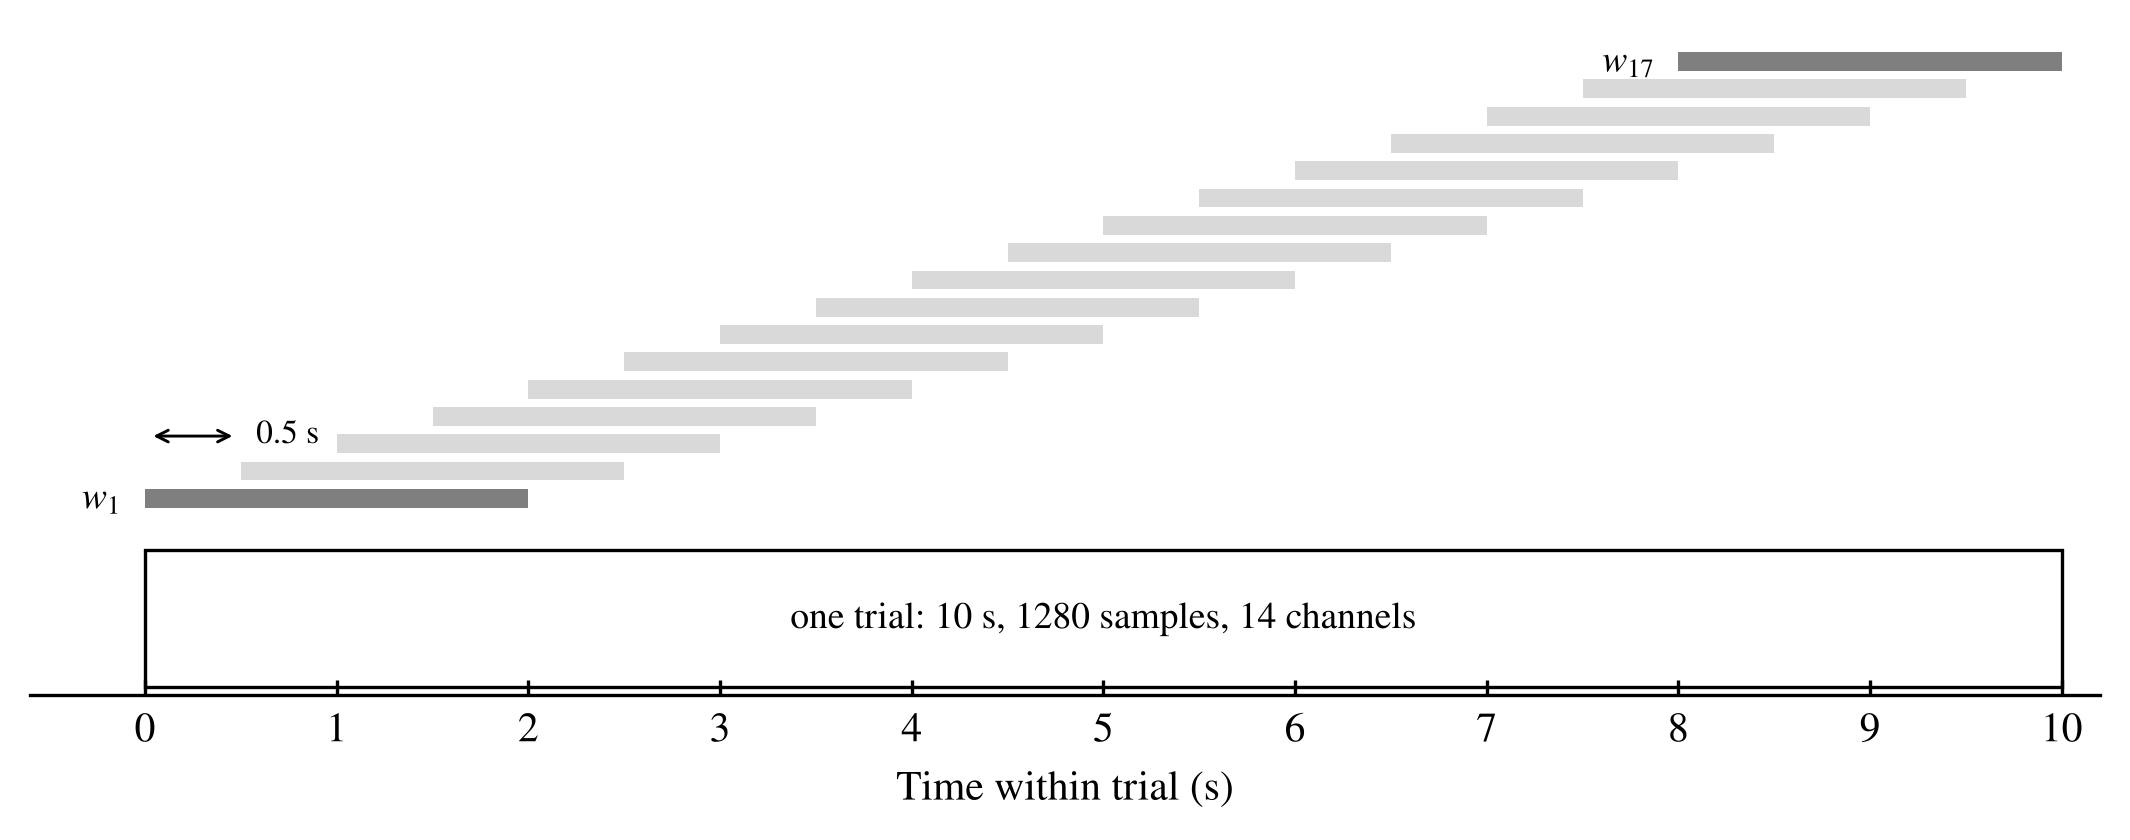
\includegraphics[width=0.85\textwidth]{figures/fig5_windowing.png}
\caption{Sliding-window segmentation of one 10~s trial into 17 windows of 2~s.}
\label{fig:windows}
\end{figure}

\subsection{Feature Extraction Overview}\label{subsec:features}

Every 2~s window becomes a fixed-length feature vector built from five families (Fig.~\ref{fig:features}): handcrafted spectral, statistical, fractal and wavelet measures; a spectrogram; a scalogram; inter-hemispheric connectivity; and the spatial covariance of the fourteen channels. The first four families give 1,666 values and the covariance family 105, so each window has 1,771 features. None of these features uses class labels.

\begin{figure}[htbp]
\centering
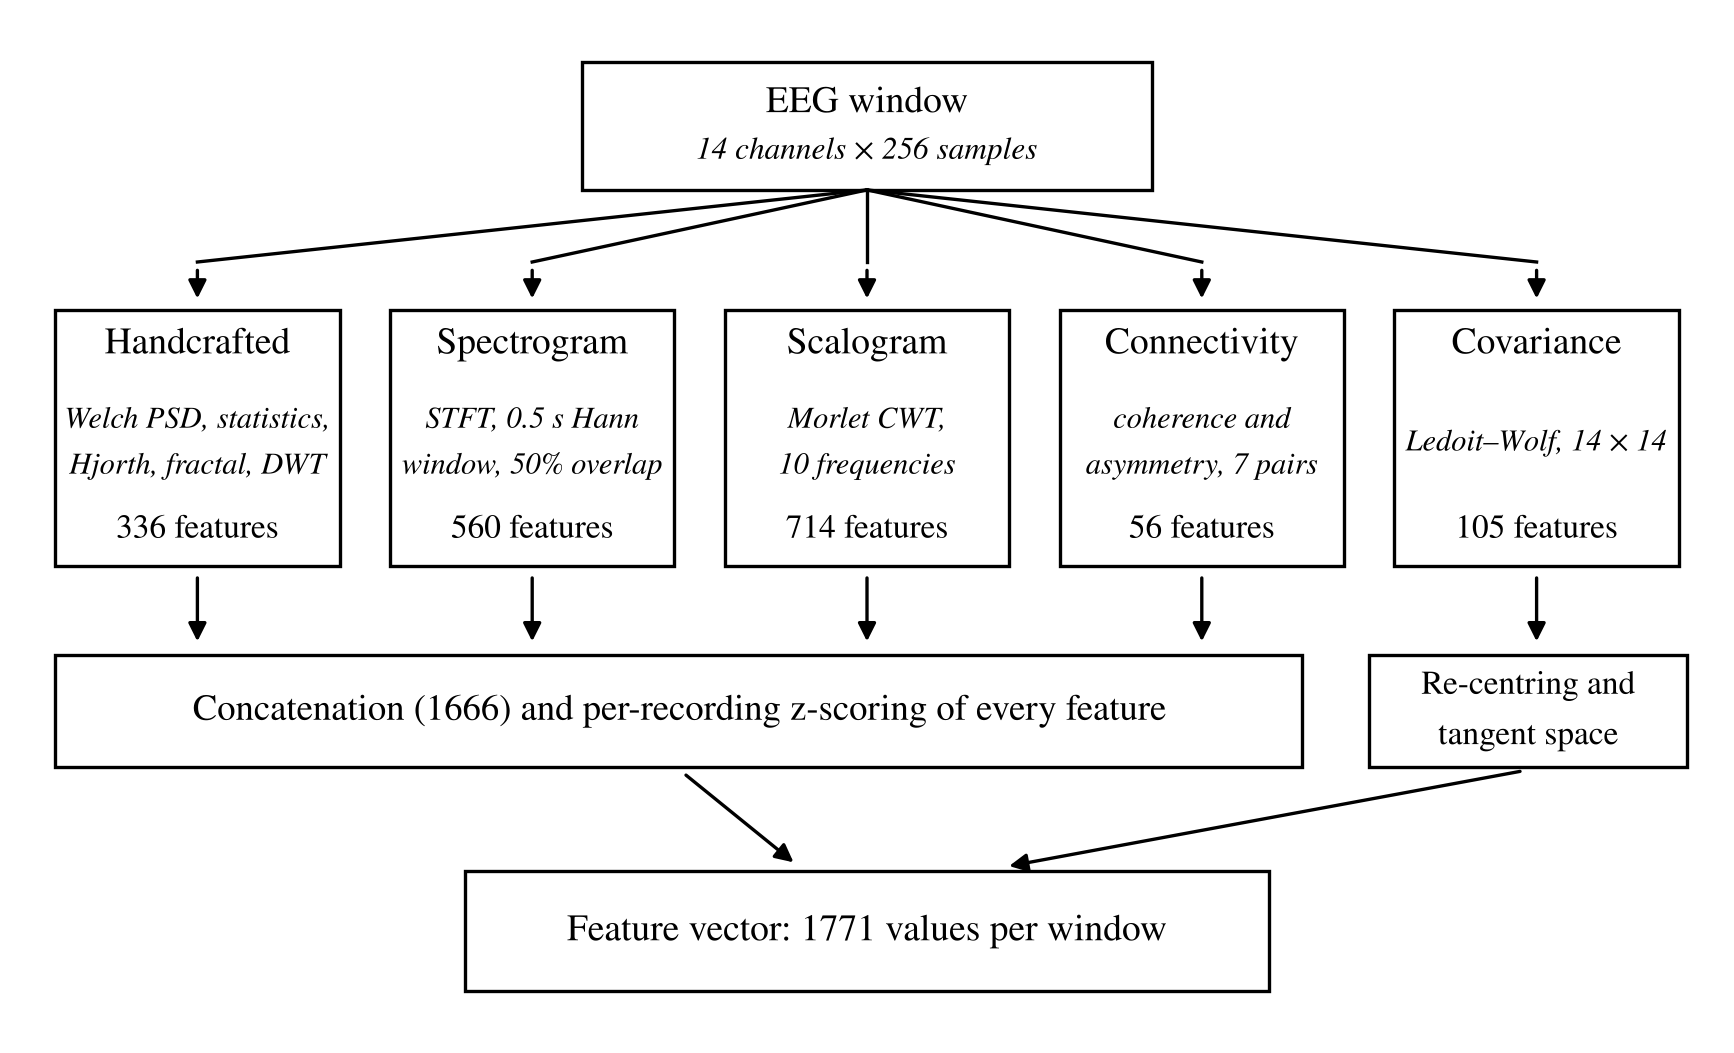
\includegraphics[width=0.9\textwidth]{figures/fig6_features.png}
\caption{The five feature families computed for each window.}
\label{fig:features}
\end{figure}

\subsection{Handcrafted Features}\label{subsec:handcrafted}

We compute 24 features for each of the 14 channels, 336 in all. The power spectral density (PSD) of each channel is estimated with Welch's method (1~s Hann segments, 50\% overlap, 1~Hz resolution), and the mean power is taken in four bands: theta (4--8~Hz), mu (8--12~Hz), beta (13--30~Hz) and gamma (30--45~Hz). For band $b$ with frequency bins $F_b$,
\begin{equation}
P_b = \frac{1}{|F_b|} \sum_{f \in F_b} \mathrm{PSD}(f).
\end{equation}
Each band is kept on a log scale, $\log(1 + P_b)$, and as relative power, $P_b / \overline{\mathrm{PSD}}$. Three ratios are added: beta/mu, mu/theta and a sensorimotor ratio $(P_\mu + P_\beta)/(P_\theta + P_\gamma)$. The time-domain group holds the variance, kurtosis, skewness and mean absolute value, together with the Hjorth mobility and complexity \citep{Hjorth1970},
\begin{equation}
\mathrm{Mobility} = \sqrt{\frac{\mathrm{var}(x')}{\mathrm{var}(x)}}, \qquad
\mathrm{Complexity} = \frac{\mathrm{Mobility}(x')}{\mathrm{Mobility}(x)}.
\end{equation}
Three non-linear measures describe how irregular the signal is: the Higuchi fractal dimension \citep{Higuchi1988} with $k_{\max} = 8$, the Petrosian fractal dimension, and the Hurst exponent from rescaled-range analysis. Last, a three-level discrete wavelet transform with the Daubechies-4 wavelet splits the window into bands of roughly 0--8, 8--16, 16--32 and 32--64~Hz, and the log energy of each band is kept.

\subsection{Spectrogram Features (STFT)}\label{subsec:stft}

Band power over a whole window tells us how much of a rhythm is present, but not when. ERD, however, is a change over time. To keep the timing we compute a spectrogram with the short-time Fourier transform,
\begin{equation}
S(t, f) = \left| \sum_{n} x[n]\, w[n - t]\, e^{-j 2\pi f n / N} \right|^2,
\end{equation}
where $w$ is a 0.5~s (64-sample) Hann window moved in 0.25~s steps. This gives 9 time frames per window and a frequency resolution of 2~Hz. For each channel and band, the power in each frame is averaged over the band and log-transformed (9 values), and the variance across frames is added to measure how unsteady the band power is. The result is $14 \times 4 \times 10 = 560$ spectrogram features.

Fig.~\ref{fig:stft} shows the mean spectrogram over all action and all imagery windows at four channels, along with their difference. At all four sites, imagery windows carry about 0.8--2~dB more power in the 8--13~Hz mu band than action windows, which fits stronger mu suppression during real movement. Action windows, for their part, show more power below 8~Hz at the frontal channel AF3 and above 30~Hz at FC5 and T8. This points to eye and head movement and to muscle activity while the participant moves.

\begin{figure}[htbp]
\centering
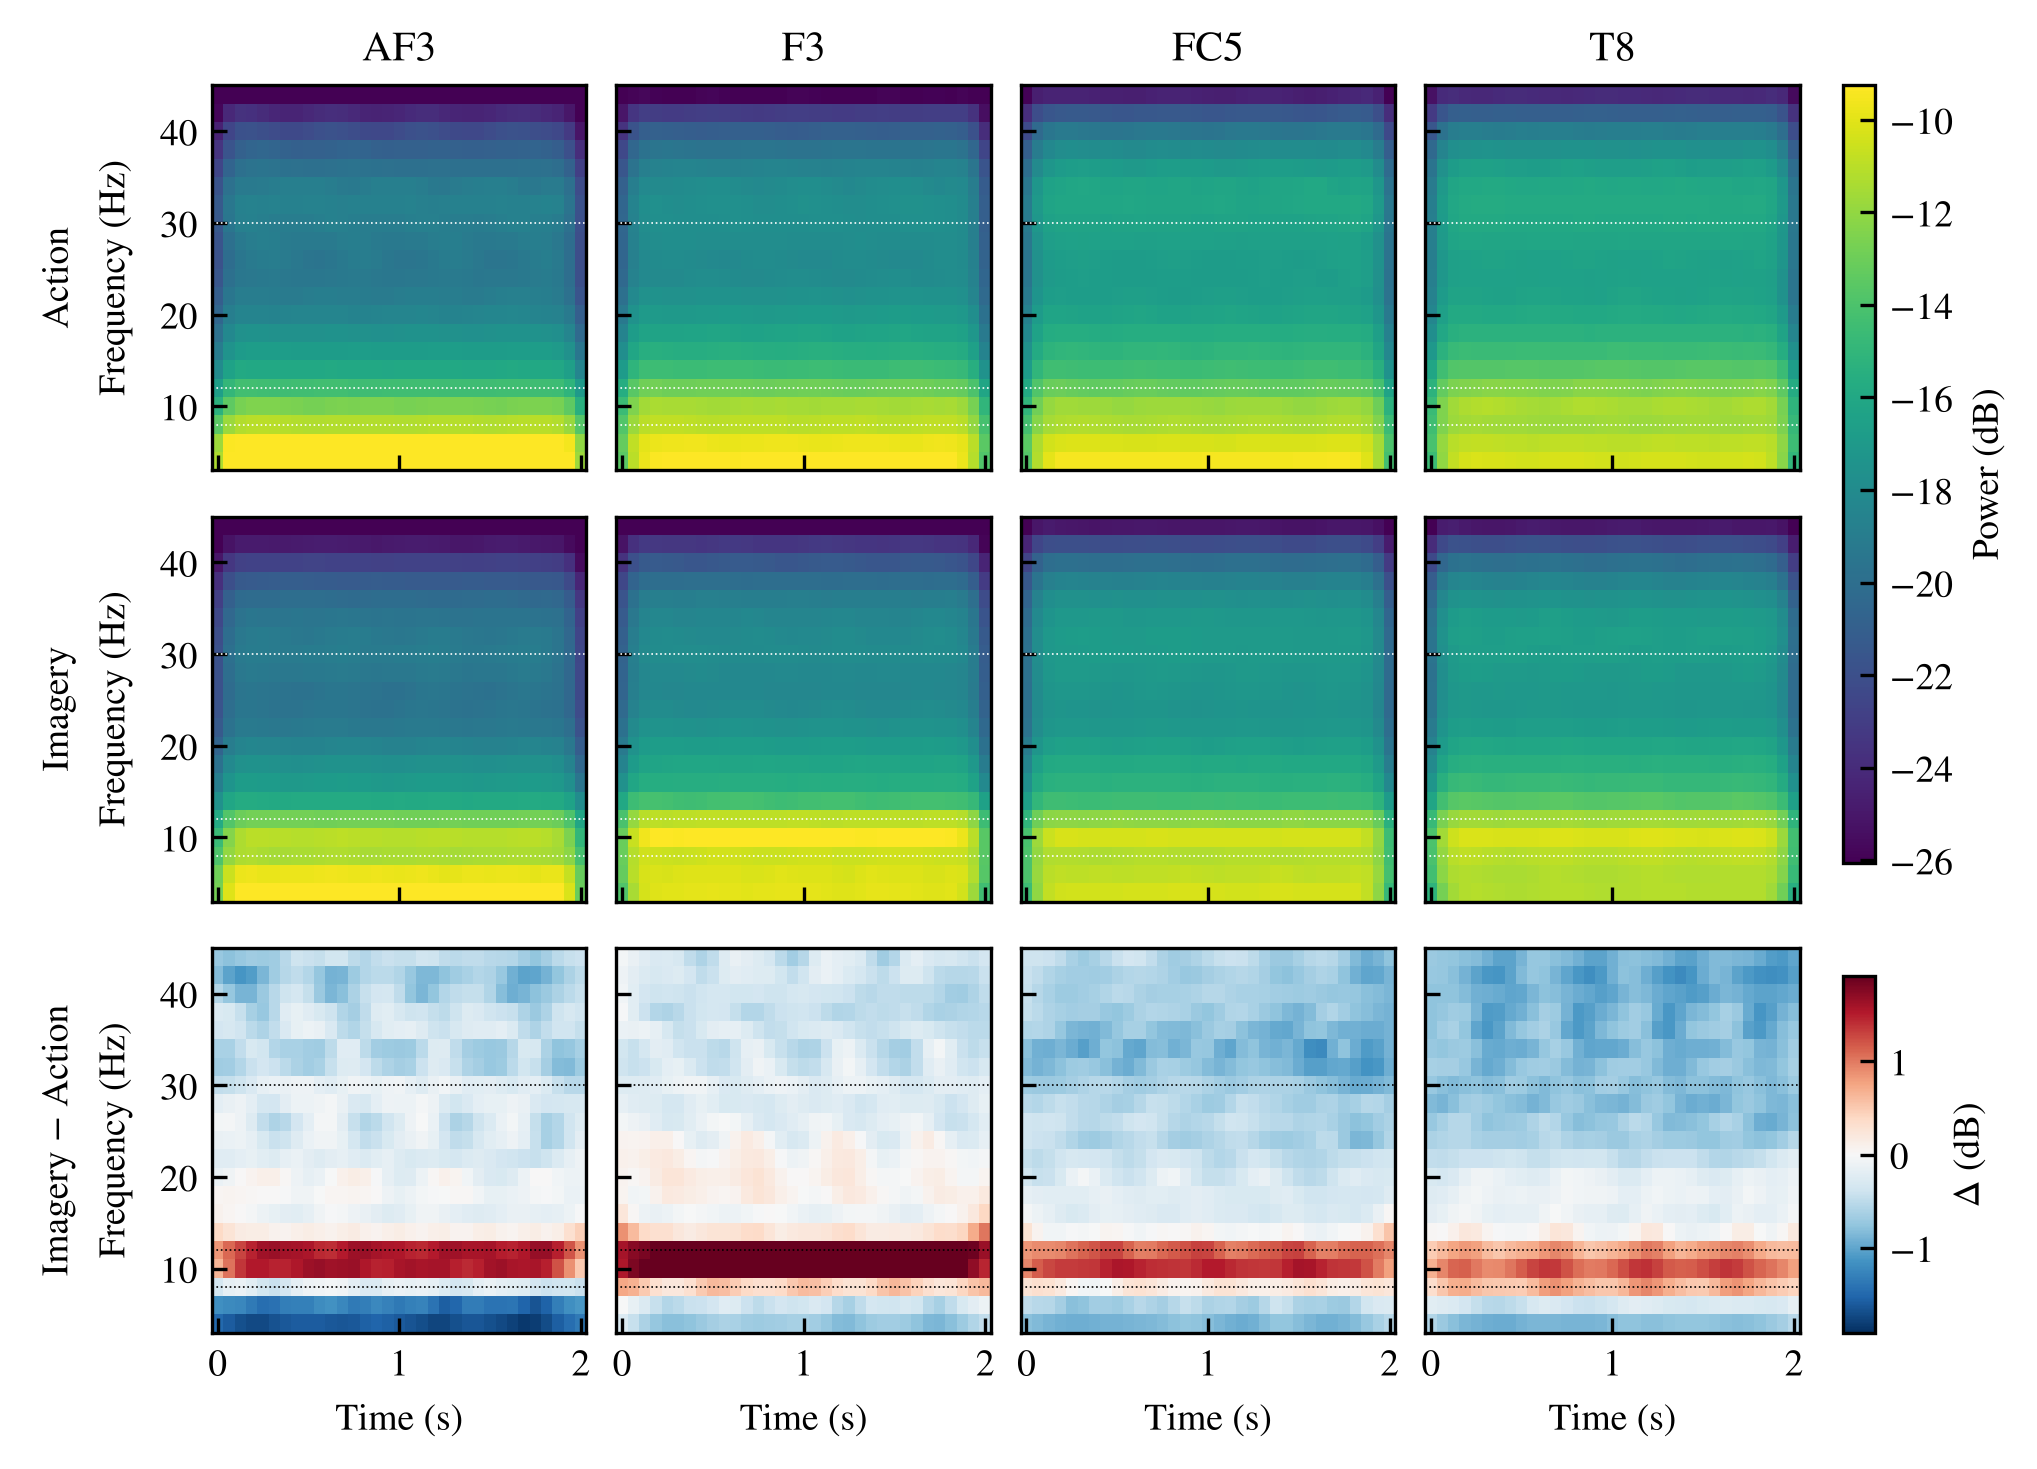
\includegraphics[width=0.9\textwidth]{figures/fig7_spectrogram.png}
\caption{Mean STFT spectrograms of action and imagery windows at AF3, F3, FC5 and T8, and their difference (imagery minus action).}
\label{fig:stft}
\end{figure}

\subsection{Scalogram Features (CWT)}\label{subsec:cwt}

The STFT uses the same window at every frequency, so it has to trade time resolution against frequency resolution. The continuous wavelet transform avoids this by stretching the analysing wavelet: short for fast rhythms, long for slow ones \citep{Torrence1998}. We use the real-valued Morlet wavelet $\psi$,
\begin{equation}
W(a, \tau) = \frac{1}{\sqrt{a}} \int x(t)\, \psi\!\left(\frac{t - \tau}{a}\right) dt, \qquad
\mathrm{Scalogram}(a,\tau) = |W(a, \tau)|^2,
\end{equation}
with scales $a$ chosen so that the centre frequencies are 5, 7, 10, 12, 15, 20, 25, 30, 35 and 40~Hz. For each channel we keep three groups of values: the log energy at each frequency in four 0.5~s segments (40 values), the ratio of high-frequency (20--40~Hz) to low-frequency (5--15~Hz) energy (1 value), and the log variance over time at each frequency (10 values). This gives $14 \times 51 = 714$ scalogram features. The mean scalograms (Fig.~\ref{fig:cwt}) show the same pattern as the spectrograms, with more mu power during imagery, but the pattern is sharper in both time and frequency, especially around 10--12~Hz.

\begin{figure}[htbp]
\centering
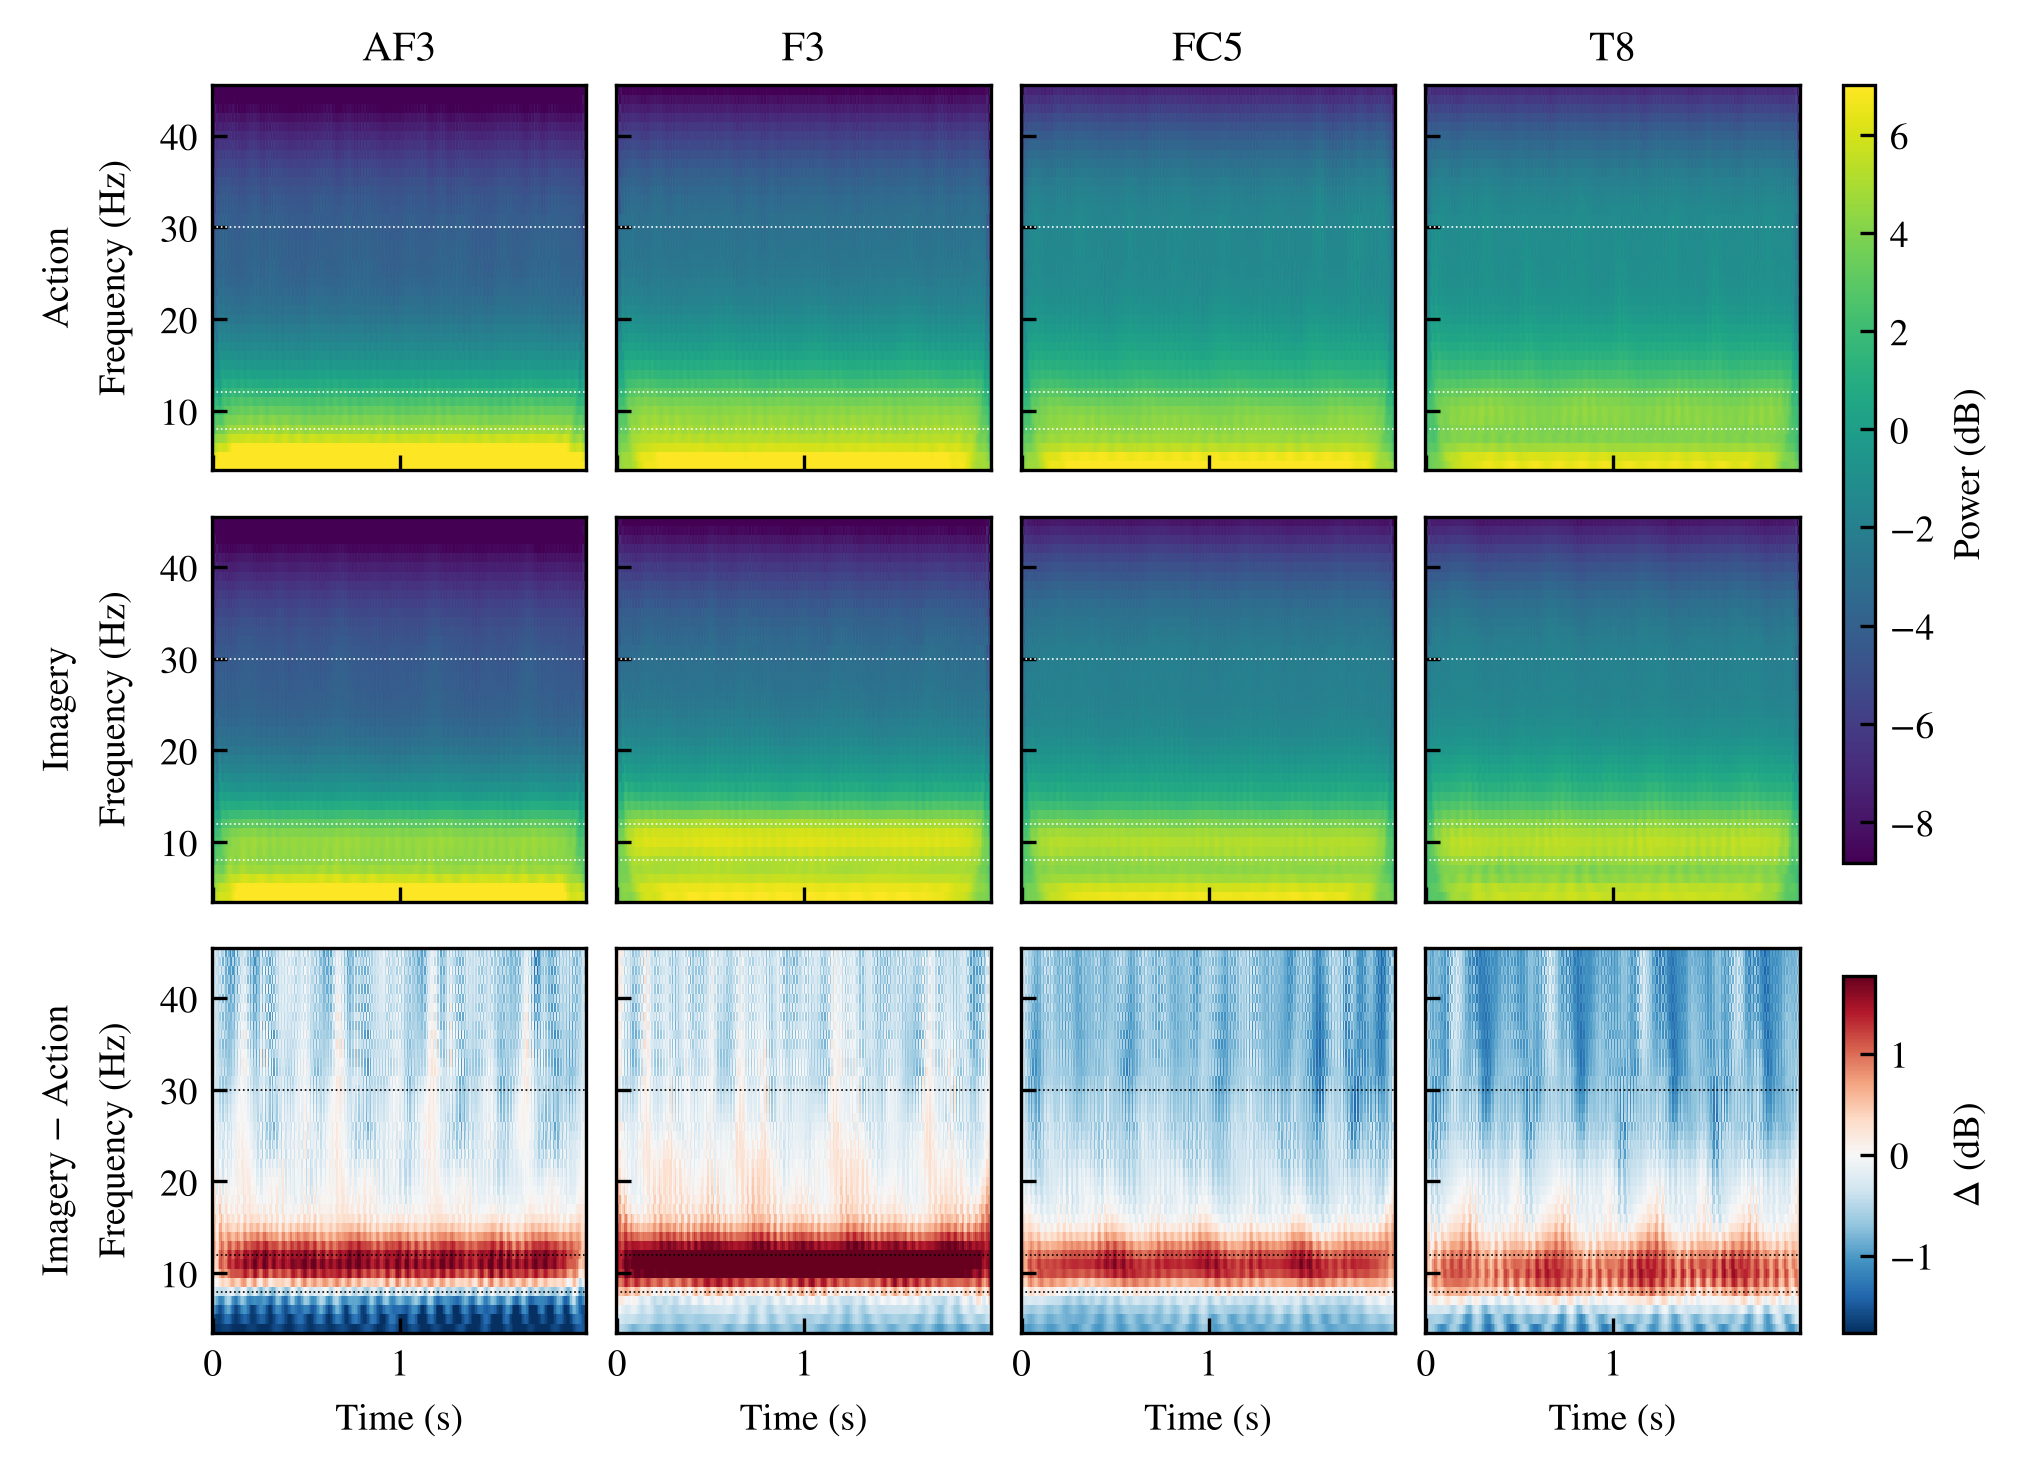
\includegraphics[width=0.9\textwidth]{figures/fig8_scalogram.png}
\caption{Mean Morlet scalograms of action and imagery windows and their difference, for the channels of Fig.~\ref{fig:stft}.}
\label{fig:cwt}
\end{figure}

\subsection{Connectivity and Covariance Features}\label{subsec:conn}

\emph{Inter-hemispheric connectivity (56 features).} Moving one side of the body mainly engages the opposite hemisphere. The 14 electrodes form seven left--right pairs (AF3--AF4, F3--F4, F7--F8, FC5--FC6, T7--T8, P7--P8, O1--O2). For each pair and band we compute the magnitude-squared coherence and the power asymmetry $\log(P_{\mathrm{left}}/P_{\mathrm{right}})$, giving $7 \times 4 \times 2 = 56$ features.

\emph{Riemannian covariance features (105 features).} For each window $X \in \mathbb{R}^{14 \times 256}$ we estimate the spatial covariance matrix
\begin{equation}
C = \frac{1}{T - 1} X X^{\top}
\end{equation}
with Ledoit--Wolf shrinkage \citep{LedoitWolf2004}, which keeps it well conditioned with only 256 samples. Covariance matrices are symmetric positive-definite and live on a Riemannian manifold \citep{Barachant2012}. To remove the offset between sessions, the matrices of each recording $r$ are re-centred on their own Riemannian mean $M_r$ \citep{Zanini2018},
\begin{equation}
\tilde{C} = M_r^{-1/2}\, C\, M_r^{-1/2},
\end{equation}
so that every recording is centred on the identity. The re-centred matrices are mapped to the tangent space at the identity, and the upper triangle is kept as a vector of $14 \times 15 / 2 = 105$ values. $M_r$ is computed from all windows of the recording, without labels.

\subsection{Subject-Wise Feature Alignment}\label{subsec:align}

Normalising the raw signal is not enough on its own. Feature values still sit in different ranges for different people; one person's mu power may simply be higher than another's. We therefore standardise each of the 1,666 non-covariance features separately for every recording $r$, using that recording's own windows:
\begin{equation}
\hat{z}_{r,j} = \frac{z_{r,j} - \mu_{r,j}}{\sigma_{r,j}}, \qquad j = 1, \dots, 1666.
\end{equation}
Together with the covariance re-centring, this puts every recording around the same reference point. The statistics pool all tasks and use no labels, so in practice a new user would need only one unlabelled calibration session.

\subsection{Hemispheric Mirror Augmentation}\label{subsec:mirror}

The EPOC X electrodes are laid out symmetrically (AF3/AF4, F7/F8, F3/F4, FC5/FC6, T7/T8, P7/P8, O1/O2). Because a limb on one side is controlled mainly by the opposite hemisphere, swapping each left electrode with its right partner gives a rough picture of the same movement made on the other side of the body. We use this to add a mirrored copy of every training window. Since every feature is computed per channel or per channel pair, the mirrored features can be built directly: per-channel handcrafted, spectrogram and scalogram columns are swapped between partners, coherence stays the same, the sign of the asymmetry is flipped, and the re-centred covariance matrix is permuted, $\tilde{C}' = P \tilde{C} P^{\top}$, before the tangent-space projection. The labels are mirrored as well (right arm $\leftrightarrow$ left arm, right leg $\leftrightarrow$ left leg, right wrist $\leftrightarrow$ left wrist), while the action/imagery condition stays as it is. Mirrored copies are added to the training folds only; test windows are never changed.

\subsection{Classification Models}\label{subsec:models}

\emph{Proposed ensemble.} The 1,771 aligned features are scaled with a standard scaler fitted on the training participants and passed to four models of different kinds (Table~\ref{tab:models}). Each model gives class probabilities for a window $w$, and the ensemble averages them with equal weights:
\begin{equation}
p_w = \frac{1}{4} \sum_{m=1}^{4} p_w^{(m)}.
\end{equation}
Linear models and tree ensembles tend to make different mistakes, so averaging them evens out some errors. We fixed the four models and their settings in advance and used them unchanged for every task.

\begin{table}[htbp]
\centering
\caption{Classifiers of the proposed ensemble.}
\label{tab:models}
\footnotesize
\begin{tabular}{@{}p{0.27\linewidth}p{0.33\linewidth}p{0.32\linewidth}@{}}
\toprule
Model & Setting & Reason for inclusion \\
\midrule
Logistic Regression (LR) & L2 penalty, $C = 0.01$ & Strongly regularised linear model \\
Linear Discriminant Analysis (LDA) & Least squares, automatic Ledoit--Wolf shrinkage & Standard EEG classifier; copes with many features \\
Extra Trees & 500 trees, $\sqrt{d}$ features per split & Non-linear, low-variance averaging of random trees \\
Histogram Gradient Boosting (HistGB) & 200 iterations, learning rate 0.05, depth 4 & Non-linear, corrects errors step by step \\
\botrule
\end{tabular}
\end{table}

\emph{Comparison models.} To put the ensemble in context, we evaluated other models on the same data and folds, at window level and without subject-wise alignment: SVM (RBF kernel, $C = 10$), Random Forest (300 trees), HistGB, Gaussian Naive Bayes, AdaBoost and shrinkage LDA. Each was applied to five feature sets: filter-bank CSP (four components in each of seven sub-bands between 4 and 40~Hz), all 1,666 features, the top-$k$ features ranked by ANOVA $F$-score ($k = 150$ for binary, 200 for multi-class), the Riemannian tangent-space features, and a combined set (CSP + all features + Riemannian). Naive Bayes and AdaBoost were left out of the multi-class runs because of their run time. We also tested Riemannian minimum distance to mean (MDM) \citep{Barachant2012}; a hierarchical model that first predicts action or imagery and then the body part; EEGNet \citep{Lawhern2018} with 8 temporal filters, depth multiplier 2 and 16 separable filters; and a CNN--LSTM with two 1-D convolution blocks followed by two LSTM layers. Both networks take the raw $14 \times 256$ windows, are trained with Adam (batch size 64) and stop early on a validation set made of 15\% of the \emph{training} participants. In every comparison model, the scaler, feature selection, CSP filters and tangent-space reference were fitted inside each fold on the training participants only.

\emph{Adding CSP to every model.} CSP is the classic feature for motor imagery, so we also checked whether it helps our own pipeline. For each fold, CSP filters (four components with Ledoit--Wolf regularisation) were fitted in each of the seven sub-bands on the training windows and their mirrored copies, the 28 log-variance features were standardised per recording, and they were appended to the 1,771 features. Eight classifiers (LR, LDA, SVM, Random Forest, Extra Trees, HistGB, AdaBoost and Naive Bayes) and the ensemble were then trained with and without these features, all with alignment, mirror augmentation and trial averaging.

\subsection{Left versus Right Motor Imagery}\label{subsec:lr}

As an extra task we asked whether the side of an imagined movement can be decoded. Only the 241 imagery trials are used, and the target is the body side (left or right) pooled over arm, leg and wrist. For this task the per-recording standardisation of Section~\ref{subsec:align} uses only that recording's imagery windows (three left and three right trials) rather than all twelve tasks; the side labels are not used. Mirror augmentation is applied as before, with the side label flipped. As a reference we also ran the standard method for this kind of problem, filter-bank CSP (seven sub-bands, four components each) followed by shrinkage LDA \citep{Ang2012}, and all eight classifiers of the CSP experiment. Significance against the 50\% chance level was tested with a one-sided binomial test.

\subsection{Trial-Level Decision and Evaluation}\label{subsec:eval}

\emph{Trial-level decision.} A working BCI decides once per task, not once per 2~s window. We therefore average the 17 window probabilities of a trial and pick the class with the highest mean:
\begin{equation}
\bar{p} = \frac{1}{17} \sum_{w=1}^{17} p_w, \qquad \hat{y} = \arg\max_c \bar{p}_c.
\end{equation}
All windows of a trial are always in the same test fold, so this averaging never mixes training and test data. We report window-level accuracy as well.

\emph{Cross-validation.} All results use person-wise GroupKFold (Fig.~\ref{fig:eval}a). Participants are split into folds and each one is tested exactly once, by a model that never saw any of their data. We used five folds for the binary tasks (9--10 test participants per fold) and three folds for the six- and twelve-class tasks (15--16 test participants per fold), which leaves enough training examples of each class. Folds are grouped by person rather than by recording, so a participant with two sessions can never be on both sides of a split.

\emph{Metrics.} Accuracy is reported as the number of correctly classified test trials pooled over all folds, and as the mean $\pm$ standard deviation across folds. Chance level is 50\% for the binary tasks, 16.67\% for six classes and 8.33\% for twelve classes.

\begin{figure}[htbp]
\centering
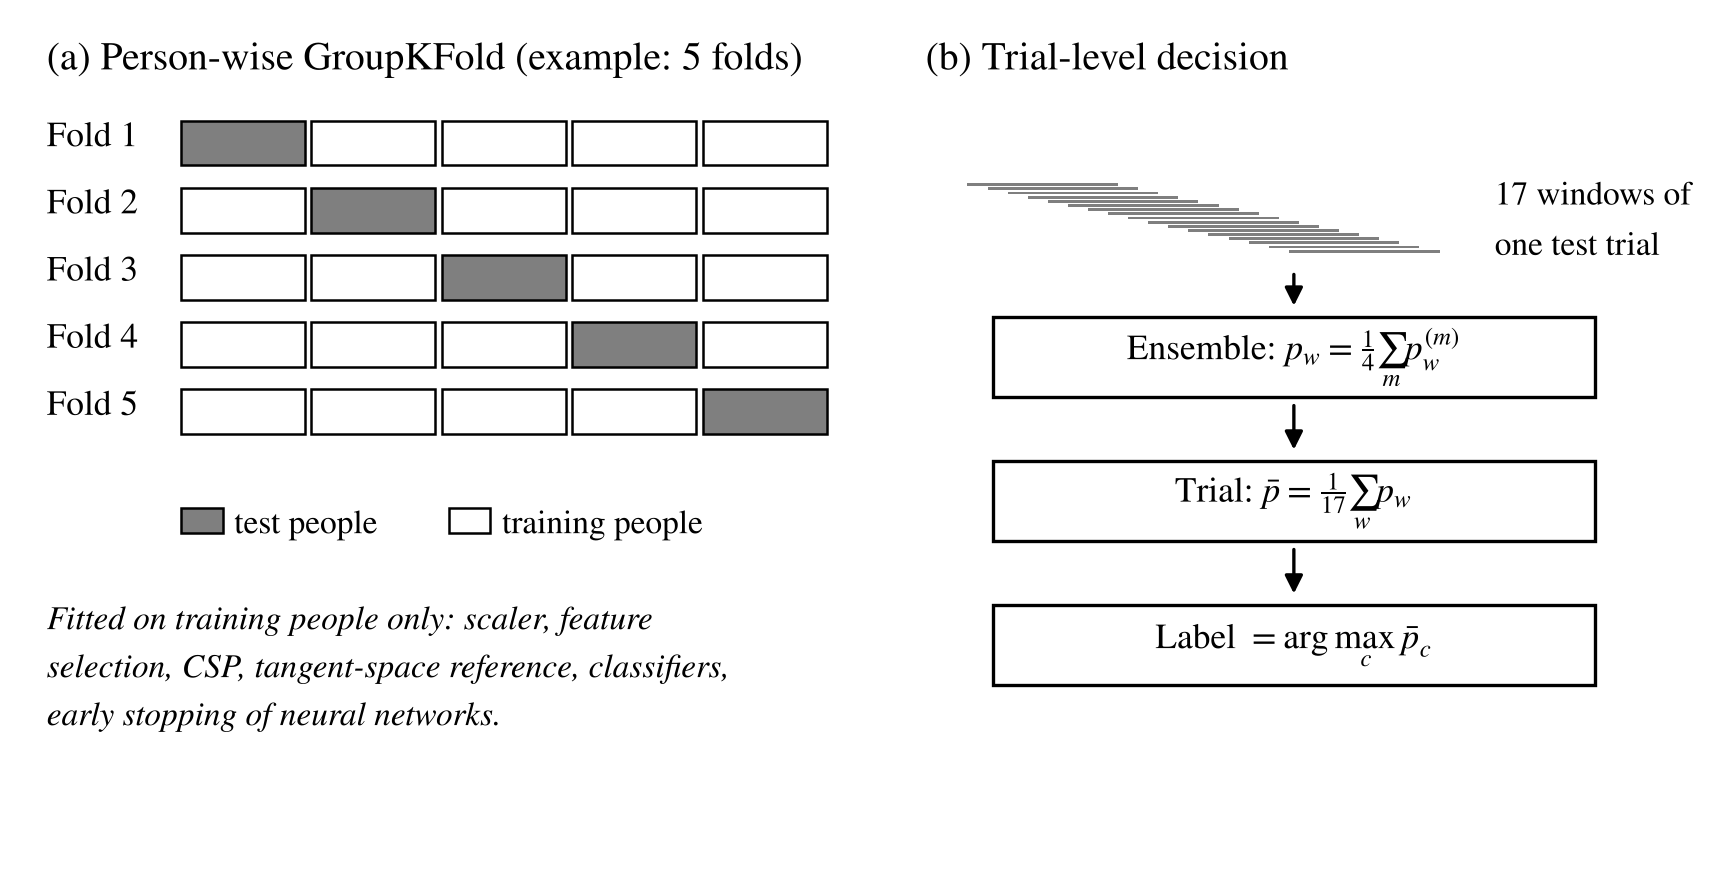
\includegraphics[width=0.9\textwidth]{figures/fig9_evaluation.png}
\caption{Evaluation scheme. (a) Person-wise GroupKFold; (b) trial-level decision.}
\label{fig:eval}
\end{figure}

\emph{Validity checks.} Four further checks were run on the final pipeline. (1) \emph{Label permutation}: the labels were shuffled across trials within each recording, and the complete pipeline, including alignment, mirror augmentation, the ensemble and trial averaging, was run three times on every task. (2) \emph{Reproducibility}: the binary pipeline was run twice with the same random seed and once each with three other seeds. (3) \emph{Onset sensitivity}: every detected onset was shifted by $\pm$2~s and part of the pipeline was re-run. (4) \emph{Nested cross-validation}: within each outer training set, an inner person-wise cross-validation picked the feature configuration and the classifier, and only that choice was then tested on the outer test participants. This last check removes the optimism that comes from comparing several set-ups on the same test people.

\FloatBarrier

%% ===================================================================
\section{Results and Discussion}\label{sec:results}

\subsection{Dataset Summary}\label{subsec:data}

Table~\ref{tab:dataset} summarises the data that reached the classifiers. After onset detection and artefact rejection, 476 trials from 47 participants remained, giving 8,092 windows. Action and imagery are almost equally represented and each of the twelve tasks has between 36 and 44 trials, so accuracy can be read directly, without any correction for class imbalance.

\begin{table}[htbp]
\centering
\caption{Summary of the processed dataset.}
\label{tab:dataset}
\begin{tabular}{@{}lc@{}}
\toprule
Parameter & Value \\
\midrule
Participants & 47 \\
EEG recordings available / used & 59 / 53 \\
Trials extracted & 636 \\
Trials rejected (amplitude / kurtosis) & 160 (25.2\%) \\
Trials retained & 476 \\
Action / imagery trials & 235 / 241 \\
Trials per task (12 classes) & 36--44 \\
EEG channels / sampling rate & 14 / 128 Hz \\
Trial length / window / stride & 10 s / 2 s / 0.5 s \\
Windows & 8,092 \\
Features per window & 1,771 \\
\botrule
\end{tabular}
\end{table}

\subsection{Main Results}\label{subsec:main}

Table~\ref{tab:main} gives the accuracy of the proposed system. Every value is subject-independent: each trial was classified by a model trained without any data from that person.

\begin{table*}[htbp]
\centering
\caption{Accuracy of the proposed ensemble with mirror augmentation (person-wise GroupKFold). Pooled = correctly classified test trials over all folds. $^\dagger$Not significant under nested cross-validation (52.28\%, Section~\ref{subsec:lrresults}).}
\label{tab:main}
\resizebox{\textwidth}{!}{%
\begin{tabular}{@{}lccccc@{}}
\toprule
Task & Classes & Chance & Trial level (pooled) & Trial level (fold mean) & Window level (fold mean) \\
\midrule
Action vs.\ imagery & 2 & 50.00\% & \textbf{80.25\%} (382/476) & 80.19 $\pm$ 6.59\% & 68.53 $\pm$ 3.59\% \\
Body part & 6 & 16.67\% & \textbf{26.68\%} (127/476) & 26.68 $\pm$ 1.79\% & 21.01 $\pm$ 0.42\% \\
Twelve tasks & 12 & 8.33\% & \textbf{21.43\%} (102/476) & 21.42 $\pm$ 1.21\% & 15.75 $\pm$ 0.83\% \\
Left vs.\ right imagery$^\dagger$ & 2 & 50.00\% & 58.09\% (140/241) & 58.10 $\pm$ 5.91\% & 52.65 $\pm$ 2.74\% \\
\botrule
\end{tabular}}
\end{table*}

Action versus imagery is by far the easiest problem. Four out of five trials from people the model had never seen were classified correctly, about 30 points above chance. The two multi-class problems are much harder, but both stay clearly above chance: body-part accuracy is 1.6 times chance and twelve-task accuracy 2.6 times. As one would expect, accuracy falls as the target becomes more specific.

Averaging over a trial helped on every task. Going from single windows to whole trials raised accuracy by 11.7 points for action versus imagery and by 5.7 points for both body part and twelve tasks. One 2~s window is noisy, and averaging 17 of them removes much of that noise. The spread between folds is large, though. Binary accuracy ranged from 71.3\% to 89.7\% depending on which participants were held out, so decoding depends heavily on the person, and differences of a point or two between methods should not be over-read.

\subsection{Contribution of the Ensemble, Alignment and Augmentation}\label{subsec:ablation}

Table~\ref{tab:ablation} compares the four ensemble members with the ensemble, and shows what happens when subject-wise alignment and mirror augmentation are switched off.

\begin{table}[htbp]
\centering
\caption{Trial-level accuracy (fold mean $\pm$ SD, \%) of the single classifiers and of the ensemble with and without alignment and augmentation. Single models were trained without augmentation.}
\label{tab:ablation}
\footnotesize
\begin{tabular}{@{}lccc@{}}
\toprule
Model & Binary & Body part (6) & Twelve tasks \\
\midrule
Logistic Regression & 79.96 $\pm$ 7.71 & 23.51 $\pm$ 1.69 & 17.67 $\pm$ 2.86 \\
LDA (shrinkage) & 76.19 $\pm$ 7.94 & 23.50 $\pm$ 3.13 & 19.55 $\pm$ 2.40 \\
Extra Trees & 77.88 $\pm$ 6.81 & 22.49 $\pm$ 1.01 & 18.92 $\pm$ 1.44 \\
HistGB & 78.74 $\pm$ 5.01 & 26.48 $\pm$ 2.91 & 19.96 $\pm$ 0.86 \\
Ensemble, no alignment, no augmentation & 70.14 $\pm$ 5.51 & 23.77 $\pm$ 2.36 & 19.34 $\pm$ 1.74 \\
Ensemble, no augmentation & 79.56 $\pm$ 6.37 & 25.60 $\pm$ 3.59 & 20.41 $\pm$ 5.59 \\
\textbf{Ensemble + mirror augmentation} & \textbf{80.19 $\pm$ 6.59} & \textbf{26.68 $\pm$ 1.79} & \textbf{21.42 $\pm$ 1.21} \\
\botrule
\end{tabular}
\end{table}

No single classifier won everywhere. Logistic regression did best on the binary problem and gradient boosting on body part. The ensemble stayed within about one point of the best single model on every task, and we kept it fixed instead of choosing a different model for each task after seeing the results.

Subject-wise alignment had the largest effect of any step. Without it, binary accuracy dropped from 79.62\% to 70.17\% (pooled, 379 vs.\ 334 of 476 trials), body part from 25.63\% to 23.74\% and twelve tasks from 20.38\% to 19.33\%. A good part of the difference between people therefore behaves like a simple shift in feature values, and per-recording standardisation takes it out. Mirror augmentation added 3, 5 and 5 correct trials for the binary, body-part and twelve-task problems (379$\to$382, 122$\to$127, 97$\to$102). These gains are small and well inside the spread across folds, but they appear on all three tasks, and the fold-to-fold variation of the multi-class tasks became much smaller (from $\pm$3.59 to $\pm$1.79 for body part and from $\pm$5.59 to $\pm$1.21 for twelve tasks).

\subsection{Comparison with Baseline Classifiers and Deep Learning}\label{subsec:baselines}

Table~\ref{tab:baselines} sets the proposed system beside the comparison models. These were evaluated per window on the same folds and with the same leakage controls, but without subject-wise alignment, augmentation or trial averaging.

\begin{table*}[htbp]
\centering
\caption{Best comparison models (window level unless stated, fold mean $\pm$ SD, \%). The neural networks and the hierarchical model used three folds for all tasks.}
\label{tab:baselines}
\resizebox{\textwidth}{!}{%
\begin{tabular}{@{}lccc@{}}
\toprule
Model & Binary & Body part (6) & Twelve tasks \\
\midrule
All features + HistGB & 64.45 $\pm$ 2.35 & 19.71 $\pm$ 0.13 & 12.90 $\pm$ 0.03 \\
CSP + all features + Riemannian, SVM & 62.89 $\pm$ 3.73 & 20.62 $\pm$ 0.59 & 14.32 $\pm$ 1.27 \\
Riemannian tangent space + SVM & 58.87 $\pm$ 2.93 & 20.70 $\pm$ 1.13 & 13.17 $\pm$ 1.78 \\
Riemannian tangent space + HistGB & 63.90 $\pm$ 4.23 & 20.27 $\pm$ 0.84 & 12.84 $\pm$ 1.20 \\
Riemannian MDM & 62.31 $\pm$ 4.64 & 19.92 $\pm$ 1.44 & 12.05 $\pm$ 1.37 \\
Hierarchical (binary $\to$ body part) & -- & -- & 13.83 $\pm$ 1.28 \\
EEGNet & 61.65 $\pm$ 2.14 & 15.94 $\pm$ 0.46 & 11.77 $\pm$ 0.55 \\
CNN--LSTM & 57.84 $\pm$ 2.08 & -- & -- \\
\textbf{Proposed (window level)} & \textbf{68.53 $\pm$ 3.59} & \textbf{21.01 $\pm$ 0.42} & \textbf{15.75 $\pm$ 0.83} \\
\textbf{Proposed (trial level)} & \textbf{80.19 $\pm$ 6.59} & \textbf{26.68 $\pm$ 1.79} & \textbf{21.42 $\pm$ 1.21} \\
\botrule
\end{tabular}}
\end{table*}

The proposed system came out on top for every task. Even at window level it beat all baselines on the binary and twelve-task problems and edged past the best body-part baselines. The strongest conventional pipelines, which combined CSP, Riemannian and handcrafted features with SVM or gradient boosting, reached 62--64\% on the binary task and about 20--21\% on body part. Riemannian classifiers were competitive throughout, especially for body part, which shows that the covariance between channels carries useful information.

Deep learning did not beat the classical pipelines. EEGNet reached 61.65\% on the binary task, close to the classical baselines, but it was at chance for body part (15.94\%) and only just above it for twelve tasks (11.77\%), and the CNN--LSTM was weaker still. With fewer than 40 training participants per fold, the networks probably did not see enough people to learn features that carry over to someone new, which matches earlier reports that deep EEG models need large training sets \citep{Roy2019,Altaheri2023}. We also noticed that the network results moved by up to about 1.5 points between runs, because GPU training is not fully deterministic, whereas the feature-based models gave the same numbers each time. The hierarchical model did not beat direct twelve-class classification either, since every mistake in its first stage is carried into the second.

\subsection{Does Adding CSP Features Help?}\label{subsec:csp}

Since FBCSP on its own was weaker than our feature set, a natural follow-up question was whether CSP features help when they are \emph{added} to it. Table~\ref{tab:csp} answers this for every classifier on three tasks.

\begin{table*}[htbp]
\centering
\caption{Trial-level accuracy (pooled, \%; correct trials in brackets) of each classifier with and without filter-bank CSP features. All models use alignment, mirror augmentation and trial averaging.}
\label{tab:csp}
\resizebox{\textwidth}{!}{%
\begin{tabular}{@{}lcccccc@{}}
\toprule
 & \multicolumn{2}{c}{Action vs.\ imagery (476)} & \multicolumn{2}{c}{Body part (476)} & \multicolumn{2}{c}{Left vs.\ right imagery (241)} \\
\cmidrule(lr){2-3}\cmidrule(lr){4-5}\cmidrule(lr){6-7}
Model & Base & + CSP & Base & + CSP & Base & + CSP \\
\midrule
\textbf{Ensemble} & \textbf{80.25} (382) & 81.30 (387) & \textbf{26.68} (127) & 25.00 (119) & 58.09 (140) & 57.26 (138) \\
Logistic Regression & 80.46 (383) & 79.83 (380) & 26.26 (125) & 26.47 (126) & 57.68 (139) & 59.34 (143) \\
LDA & 80.25 (382) & 80.04 (381) & 23.95 (114) & 24.16 (115) & 56.85 (137) & 59.34 (143) \\
HistGB & 79.20 (377) & 80.04 (381) & 24.58 (117) & 24.16 (115) & 50.21 (121) & 53.11 (128) \\
SVM (RBF) & 77.94 (371) & 76.89 (366) & 25.21 (120) & 26.89 (128) & 54.36 (131) & 54.77 (132) \\
Extra Trees & 77.94 (371) & 78.99 (376) & 19.33 (92) & 21.64 (103) & 50.62 (122) & 51.45 (124) \\
Random Forest & 77.52 (369) & 78.57 (374) & 19.96 (95) & 20.59 (98) & 44.81 (108) & 43.57 (105) \\
AdaBoost & 78.78 (375) & 79.83 (380) & 19.33 (92) & 20.80 (99) & 48.55 (117) & 54.36 (131) \\
Naive Bayes & 73.11 (348) & 72.90 (347) & 19.54 (93) & 19.33 (92) & 45.23 (109) & 48.13 (116) \\
\botrule
\end{tabular}}
\end{table*}

The short answer is: not much, and not in a consistent direction. On action versus imagery, CSP added about one point to the tree models (HistGB, Extra Trees, Random Forest, AdaBoost) and took up to one point from logistic regression and SVM. On body part, it helped Extra Trees (+2.3 points) and SVM (+1.7 points, the best single result at 26.89\%) but lowered the ensemble from 26.68\% to 25.00\%. On left versus right, it gave logistic regression and LDA four extra trials each (59.34\%) and AdaBoost almost six points, but these models were still close to chance, and the result for the ensemble went down slightly. Taken over all three tasks, the ensemble gained five trials on the binary problem (81.30\%) and lost eight on body part and two on left versus right. All of these changes are about the size of the spread between folds, or smaller, and they point in different directions for different tasks. We therefore kept the pipeline without CSP and treat it as an optional extra rather than an improvement.

We think there are two reasons CSP adds so little here. First, a CSP feature is the log-variance of a spatially filtered signal, which is a weighted combination of band power and inter-channel covariance; our set already contains band power for every channel in every band and the full covariance matrix in tangent space, so most of what CSP finds is already present. Second, CSP filters are fitted on the training participants, and spatial patterns transfer poorly between people when only 14 electrodes are available and none of them lies over the central motor strip. The tree models gain a little because CSP hands them a compact summary of information that is spread over hundreds of columns in the full feature set.

\subsection{Spectrogram versus Scalogram Features}\label{subsec:families}

To measure what each feature family is worth on its own, we re-ran the ensemble pipeline (with alignment and trial averaging, without mirror augmentation) using one family at a time (Fig.~\ref{fig:families}, Table~\ref{tab:families}).

\begin{figure}[htbp]
\centering
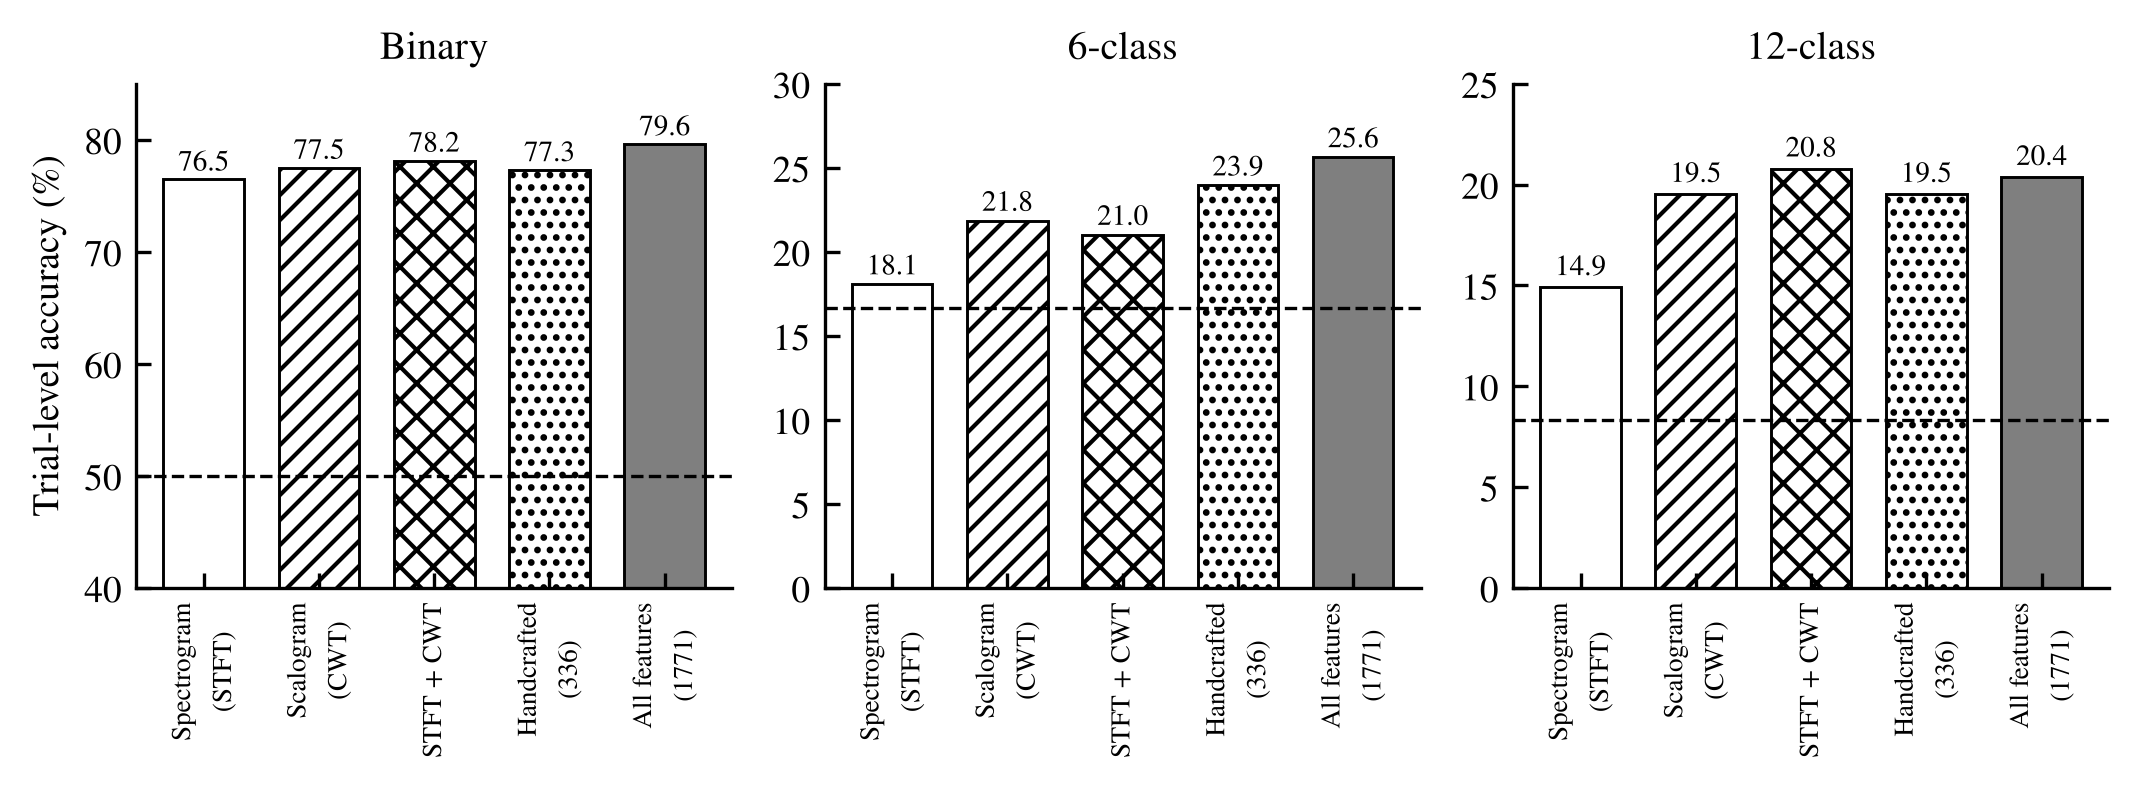
\includegraphics[width=\textwidth]{figures/fig10_feature_families.png}
\caption{Trial-level accuracy of the ensemble with a single feature family (without mirror augmentation). Dashed line: chance level.}
\label{fig:families}
\end{figure}

\begin{table}[htbp]
\centering
\caption{Trial-level accuracy (pooled, \%; correct trials in brackets) with single feature families, without mirror augmentation.}
\label{tab:families}
\footnotesize
\begin{tabular}{@{}lcccc@{}}
\toprule
Features & Number & Binary & Body part (6) & Twelve tasks \\
\midrule
Spectrogram (STFT) & 560 & 76.47 (364) & 18.07 (86) & 14.92 (71) \\
Scalogram (CWT) & 714 & 77.52 (369) & 21.85 (104) & 19.54 (93) \\
STFT + CWT & 1,274 & 78.15 (372) & 21.01 (100) & 20.80 (99) \\
Handcrafted & 336 & 77.31 (368) & 23.95 (114) & 19.54 (93) \\
All features & 1,771 & \textbf{79.62} (379) & \textbf{25.63} (122) & 20.38 (97) \\
\botrule
\end{tabular}
\end{table}

The scalogram beat the spectrogram on all three tasks. The gap was small for the binary task (1.05 points) but large for body part (3.78) and twelve tasks (4.62); with the spectrogram alone, body-part accuracy was barely above chance. This is what the theory in Section~\ref{subsec:cwt} predicts. The STFT uses a single 0.5~s window, so its frequency resolution is only 2~Hz and the mu and beta bands blur together, while the Morlet wavelet adapts its length to each frequency and resolves the 8--13~Hz rhythm more sharply. The difference maps in Figs.~\ref{fig:stft} and~\ref{fig:cwt} show the same thing. On its own the scalogram matched the 336 handcrafted features on the binary and twelve-task problems, and STFT plus CWT gave the best twelve-task accuracy in this comparison (20.80\%). For body part, adding the handcrafted, connectivity and covariance features lifted accuracy from about 21\% to 25.63\%, so telling limbs apart also relies on spatial and statistical information that the time--frequency maps do not capture.

\subsection{Most Informative Features}\label{subsec:importance}

To see which features separate action from imagery, we computed an ANOVA $F$-score for every feature on the training participants of each fold and averaged it over the five folds (Fig.~\ref{fig:importance}).

\begin{figure}[htbp]
\centering
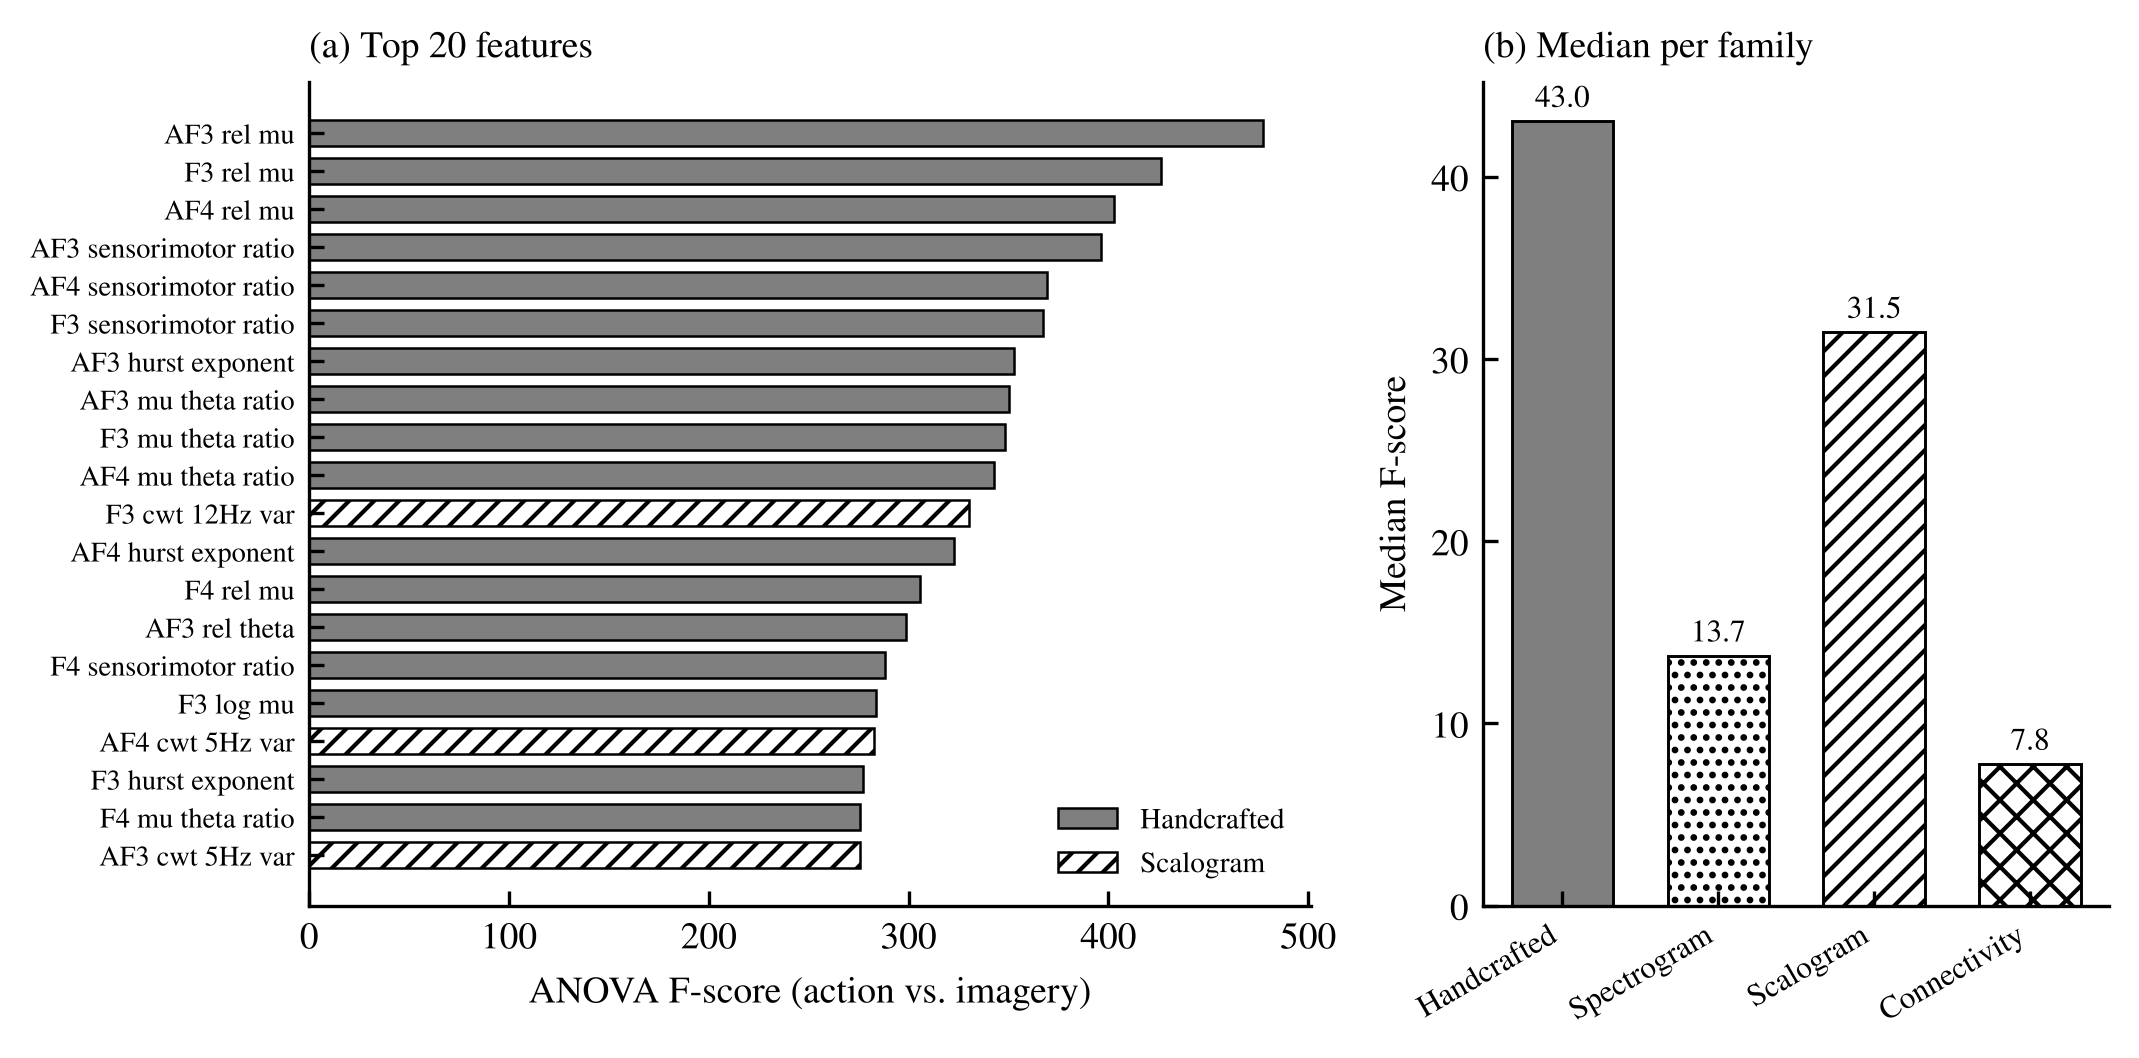
\includegraphics[width=\textwidth]{figures/fig12_feature_importance.png}
\caption{Discriminative power of the features for action versus imagery. (a) The 20 features with the highest ANOVA $F$-score; (b) median $F$-score per family.}
\label{fig:importance}
\end{figure}

Almost all of the strongest features are mu-band measures: relative mu power, the mu/theta ratio and the sensorimotor ratio. This agrees with the spectrogram and scalogram maps, where imagery trials had more mu power than action trials, the expected sign of stronger desynchronisation during real movement \citep{Pfurtscheller2001}. Three scalogram features, the temporal variance of wavelet energy at 12~Hz and 5~Hz, also make the top 20. By family, the handcrafted features have the highest median $F$-score (43.0), followed by the scalogram (31.5), the spectrogram (13.7) and connectivity (7.8).

There is one important caveat. The strongest features come from the frontal electrodes AF3, AF4, F3 and F4, not from the central motor cortex, which the EPOC X does not cover. Frontal sites are also the ones most exposed to eye movement and muscle activity, and Figs.~\ref{fig:stft} and~\ref{fig:cwt} show extra low-frequency power at AF3 and extra high-frequency power at FC5 and T8 during action trials. Part of the action-versus-imagery accuracy is therefore probably due to the side effects of moving (eye, head and muscle activity) rather than to cortical activity alone. Separating the two would need ICA-based artefact removal or EMG reference channels.

\subsection{Error Analysis}\label{subsec:errors}

Fig.~\ref{fig:confusion} shows the confusion matrices of the proposed system, pooled over all test folds. On the binary task the errors were fairly balanced: 77.0\% of action trials and 83.4\% of imagery trials were recognised. For body part, the classifier was better at telling \emph{which limb} than \emph{which side}. The arm, leg or wrist was identified in 46.0\% of trials (chance 33.3\%), but the side in only 54.6\% (chance 50\%). Right arm (37.8\%) and right wrist (31.0\%) were recognised best and left wrist worst (13.5\%). Confusing left and right is not surprising with this headset, because lateralised motor activity is strongest over C3 and C4, and the EPOC X has no electrodes there. In the twelve-task problem, the action/imagery part of the label was right in 78.2\% of trials but the body part in only 25.8\%, so most twelve-task errors come from the body part, not the condition.

\begin{figure}[htbp]
\centering
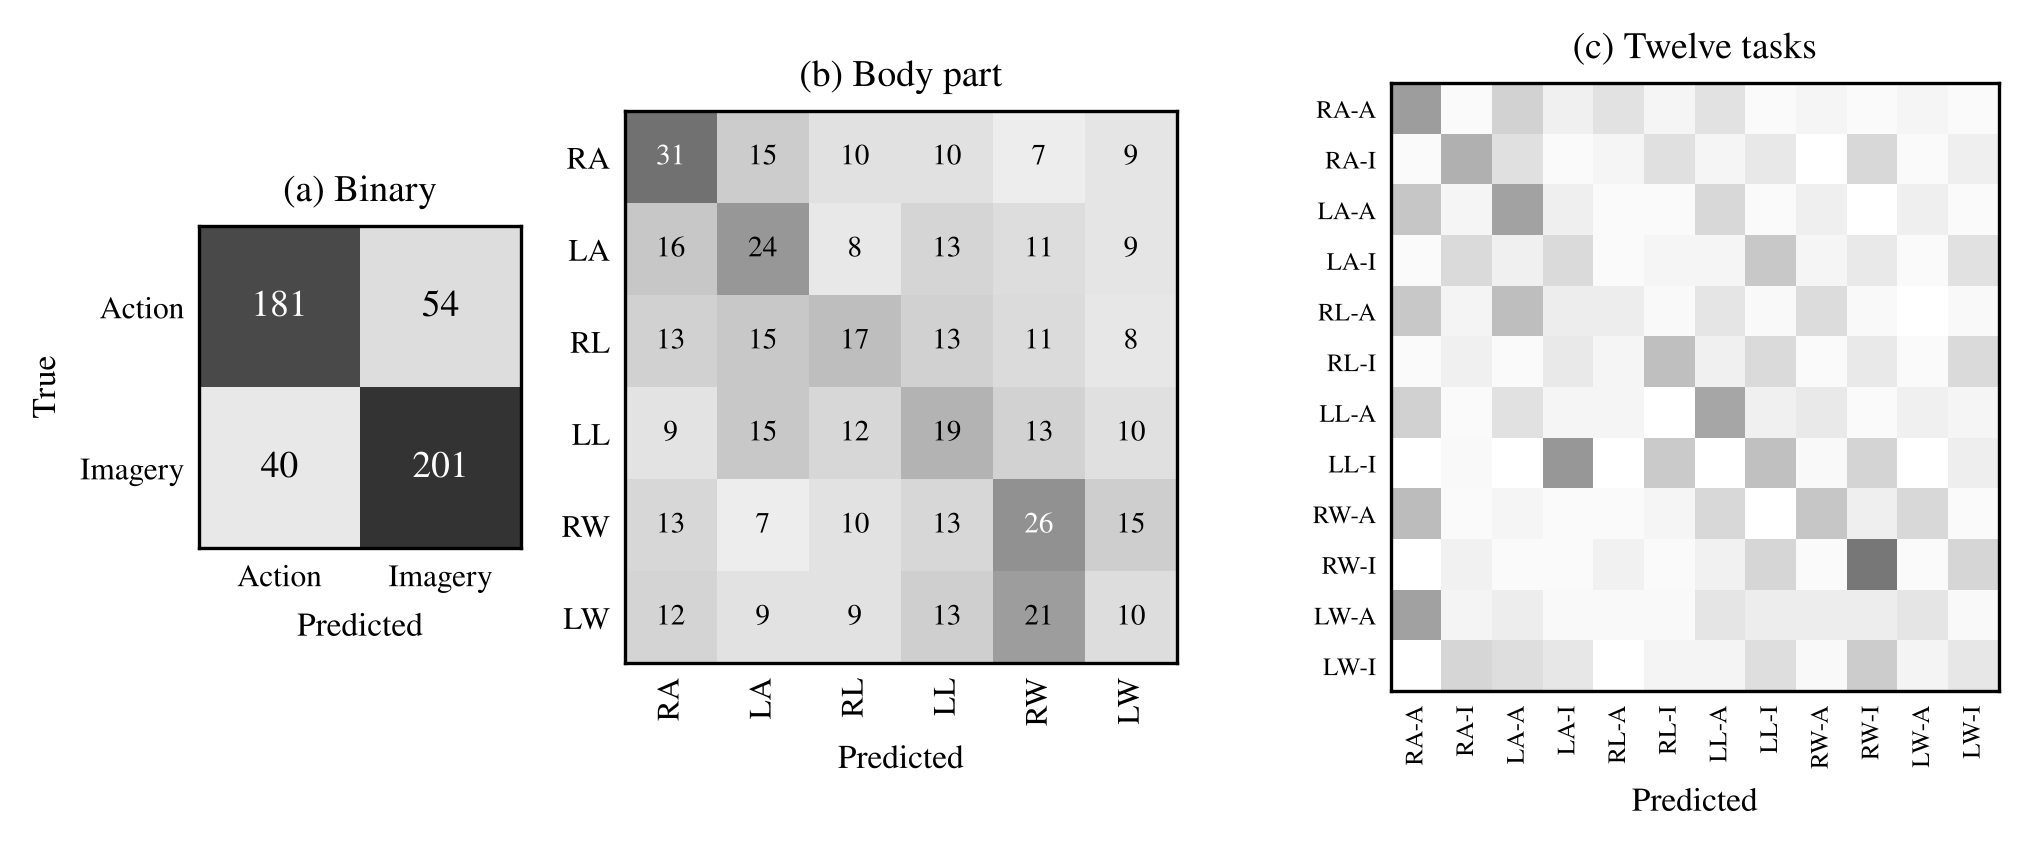
\includegraphics[width=\textwidth]{figures/fig11_confusion.png}
\caption{Trial-level confusion matrices pooled over all test folds: (a) action vs.\ imagery, (b) body part, (c) twelve tasks.}
\label{fig:confusion}
\end{figure}

\subsection{Left versus Right Motor Imagery}\label{subsec:lrresults}

Table~\ref{tab:lr} lists the results for left versus right imagery.

\begin{table}[htbp]
\centering
\caption{Left versus right motor imagery (imagery trials only, trial level, person-wise five-fold GroupKFold). Chance = 50\%; with 241 trials, 55.6\% is needed for $p < 0.05$.}
\label{tab:lr}
\footnotesize
\begin{tabular}{@{}lccc@{}}
\toprule
Method & Correct & Accuracy & $p$ (binomial) \\
\midrule
FBCSP + LDA (standard baseline) & 127/241 & 52.70\% & 0.22 \\
Ensemble, standard calibration + mirror & 129/241 & 53.53\% & 0.15 \\
Ensemble, imagery-only calibration + mirror & 140/241 & 58.09\% & 0.007 \\
\quad arm only & 60/81 & 74.07\% & $<$0.001 \\
\quad leg only & 46/78 & 58.97\% & 0.07 \\
\quad wrist only & 48/82 & 58.54\% & 0.08 \\
\midrule
\textbf{Nested cross-validation} (set-up chosen inside each fold) & \textbf{126/241} & \textbf{52.28\%} & \textbf{0.26} \\
\botrule
\end{tabular}
\end{table}

Deciding which side an imagined movement belonged to was the hardest problem in this study. The standard FBCSP + LDA method, which works well for left/right hand imagery with research-grade equipment, stayed at chance (52.70\%). Our ensemble reached 58.09\% ($p = 0.007$), but only when each person's features were calibrated on their imagery trials alone and mirror augmentation was used. Arm imagery looked by far the most separable (74.07\%, 60 of 81 trials), while leg and wrist were not significant on their own. Across the eight classifiers of Table~\ref{tab:csp}, the linear models did best (logistic regression 57.68\%, LDA 56.85\%, SVM 54.36\%), and the tree models and Naive Bayes stayed between 45\% and 51\%. A difference between left and right imagery is a small, roughly linear power difference between the hemispheres, which linear models capture more easily than tree ensembles trained on only about 190 trials per fold.

The 58.09\% figure, however, does not survive a stricter test. The imagery-only calibration was picked after comparing several set-ups on the same test participants, and that choice itself can inflate the score. In nested cross-validation, where the calibration, augmentation and classifier were chosen using only the training participants of each fold, accuracy fell to 52.28\% (126/241, $p = 0.26$). The inner loop did not settle on one set-up either: it picked a different combination of calibration and model in almost every fold (imagery-only calibration in three folds, standard calibration in two; logistic regression, LDA or Extra Trees). The per-limb figures come from the same selected set-up and are likely optimistic too. We therefore conclude that, with this headset and protocol, the side of an imagined movement cannot yet be decoded reliably in people the model has not seen.

Two further points support caution. In our protocol the right-side task always came 30~s before the matching left-side task, so slow changes during a session, such as electrodes drying or attention drifting, could help to separate ``right'' from ``left''. The arm pair comes at the start of the session, where such drift is likely strongest. A recording with left and right imagery in random order, more repetitions per person and electrodes over C3 and C4 is needed before any claim about lateralised imagery can be made.

\subsection{Validity Checks}\label{subsec:validity}

Because an early version of this work reported inflated accuracies (Section~\ref{subsec:design}), we tested the final pipeline for hidden leaks in several ways (Table~\ref{tab:validity}).

\begin{table}[htbp]
\centering
\caption{Validity checks on the final pipeline (trial-level accuracy, \%).}
\label{tab:validity}
\footnotesize
\begin{tabular}{@{}p{0.30\linewidth}p{0.36\linewidth}p{0.24\linewidth}@{}}
\toprule
Check & Result & Reference \\
\midrule
Shuffled labels, action vs.\ imagery & 54.62, 52.10, 50.21 & Chance 50; real 80.25 \\
Shuffled labels, body part & 18.07, 19.33, 17.02 & Chance 16.67; real 26.68 \\
Shuffled labels, twelve tasks & 10.50, 7.98, 8.19 & Chance 8.33; real 21.43 \\
Shuffled labels, left vs.\ right & 45.64, 43.57, 51.04 & Chance 50; real 58.09 \\
\addlinespace
Same seed, two runs (binary) & 382/476 and 382/476 & Identical \\
Three other seeds (binary) & 384, 384, 386 of 476 & Mean of 5 runs 80.59 $\pm$ 0.35 \\
\addlinespace
Nested CV, left vs.\ right & 126/241 = 52.28 & Standard CV 58.09 \\
\botrule
\end{tabular}
\end{table}

\emph{Fold integrity.} In every fold of every task, no participant, recording or trial appeared in both the training and the test set, and no EEG file was present twice under different names.

\emph{Label permutation.} A pipeline that leaks information keeps scoring above chance even when the labels are meaningless. Ours did not: with shuffled labels, all four tasks fell to the level expected from guessing (Table~\ref{tab:validity}).

\emph{Reproducibility.} Running the binary pipeline twice with the same seed gave exactly the same 382 correct trials, and three other seeds gave 384, 384 and 386. The small differences come from the random parts of the tree models, not from anything learned between runs, so repeated runs do not creep upwards. Over the five runs the binary accuracy was 80.59 $\pm$ 0.35\%.

\emph{Nested cross-validation.} For left versus right imagery, choosing the set-up inside each fold lowered accuracy from 58.09\% to 52.28\%, which is no longer significant (Section~\ref{subsec:lrresults}).

\emph{Sensitivity to the onset estimate.} Each onset was chosen to maximise the action--imagery difference in head motion, so it could in principle favour the binary task. We shifted every onset by $\pm$2~s and repeated the classification with the faster feature families (spectrogram, scalogram, connectivity and covariance; Table~\ref{tab:onsetsens}).

\begin{table}[htbp]
\centering
\caption{Trial-level accuracy after shifting all detected onsets (spectrogram, scalogram, connectivity and covariance features, without mirror augmentation).}
\label{tab:onsetsens}
\footnotesize
\begin{tabular}{@{}lcc@{}}
\toprule
Onset shift & Binary & Body part (6) \\
\midrule
$-2$ s & 76.16\% (361/474) & 27.00\% (128/474) \\
0 s (detected) & 79.20\% (377/476) & 26.89\% (128/476) \\
$+2$ s & 75.85\% (355/468) & 25.00\% (117/468) \\
\botrule
\end{tabular}
\end{table}

Body-part accuracy barely moved, but binary accuracy fell by about 3 points when the onset was shifted. Some of this drop is expected, since a shifted window takes in 2~s of rest or of the next task, but it also means the binary result may be optimistic by up to about 3 points. Even in the worst case it stays above 75\%, so our conclusions do not change.

\subsection{Effect of Evaluation Design}\label{subsec:design}

An early version of this pipeline reported accuracies above 94\%. Those numbers came from random window-level splits, with feature selection and spatial filters fitted on all of the data. Overlapping windows from the same trial and the same person ended up on both sides of the split, so the model could recognise the person, or even the trial, instead of the task. Once every learned step was restricted to the training participants and folds were grouped by person, accuracy fell to realistic levels. How a model is evaluated can matter more than which classifier is used, and person-wise grouping should be standard whenever the goal is a BCI that works for new users \citep{Lotte2018}.

The left-versus-right result teaches a related lesson. Even with strict person-wise folds, picking the best of several set-ups on the same test people raised the score from about 52\% to 58\%. Nested cross-validation is cheap insurance against this. A second, less obvious source of error was the trial timing: with a fixed 15~s onset, most windows carried the label of the task after the one actually being performed. The motion-guided onset detection of Section~\ref{subsec:onset} fixes this at the source, and a similar check is worth doing for any dataset whose stimulus markers are not stored with the EEG.

\subsection{Limitations}\label{subsec:limits}

Several limitations should be kept in mind. First, the Emotiv EPOC X has no electrodes over the central motor strip (C3, Cz, C4), which limits body-part and left--right decoding; a headset with central coverage would probably help most for these tasks. Second, the dataset holds 476 trials, about 40 per task. Sliding windows increase the number of training samples but not the number of independent trials or people. Third, artefact handling relies on filtering and trial rejection, which removed a quarter of the trials; ICA could keep more data and help to separate cortical activity from eye and muscle activity, which probably contributes to the binary result. Fourth, every participant did the tasks in the same order, so slow drift, fatigue or time-on-task may be partly mixed up with the task label, most of all for left versus right. Fifth, the ensemble and its settings were fixed before testing, but they were developed on this same group of participants without a separate held-out group, so the multi-class results may be slightly optimistic. Finally, all results are offline. Subject-wise alignment assumes one unlabelled calibration session for each new user, and an online test with real-time feedback is still to be done.

\FloatBarrier
%% ===================================================================
\section{Conclusion}\label{sec:conclusion}

We have presented a subject-independent pipeline for classifying motor action and motor imagery from a 14-channel consumer-grade Emotiv EPOC X. Using EEG from 47 participants who performed and imagined six limb movements, we analysed the same recordings at several levels of difficulty. Three steps mattered most: recovering the real trial onsets from the headset's motion sensor, which fixed a timing error that had mislabelled most trials in our earlier attempts; standardising features within each recording without labels, which removed much of the difference between people; and averaging the predictions of all windows in a trial, which gave far more reliable decisions than single 2~s windows.

With these steps and a four-model ensemble trained with hemispheric mirror augmentation, the system reached 80.25\% for action versus imagery, 26.68\% for six body parts and 21.43\% for all twelve tasks on people never seen during training, all well above chance. Shuffled-label tests fell to chance on every task, repeated runs gave nearly identical results, and the system beat CSP, Riemannian and deep-learning baselines tested under the same conditions. Adding CSP features changed the ensemble's accuracy by less than two points, upwards on one task and downwards on the other two, because our feature set already covers most of the band-power and covariance information that CSP extracts. Among the time--frequency representations, the Morlet scalogram was consistently more useful than the STFT spectrogram, thanks to its sharper view of the mu rhythm.

The study also shows where a low-cost headset falls short. Left versus right imagery reached 58.09\% in standard cross-validation but only 52.28\% under nested cross-validation, and identifying the limb was much harder than telling movement from imagery. Without electrodes over the central motor strip, these finer distinctions remain out of reach. Future work will use recordings with randomised task order, more imagery repetitions and better electrode coverage, ICA-based removal of eye and muscle activity, and online testing with real-time feedback.

\section{Data availability}
Data will be available upon request.

\section{Author Contributions}
All authors read and approved the final manuscript.

\section{Funding}
All necessary funding, including support for open access publication, is provided by Amrita Vishwa Vidyapeetham, India.

\bibliography{bibliography}

\end{document}
